\chapter{AdaptativeSR: pruning-based Topology Refinement of 3D Mesh with 2D Masks
}
\label{chapter:appendix-adaptativeSR}

%\minitoc
\chapterwithfigures{\nameref*{chapter:appendix-adaptativesr}}
\chapterwithtables{\nameref*{chapter:appendix-adaptativesr}}

\ifthenelse{\boolean{skipAppendix}}{\endinput}{}


Image-based 3D reconstruction has achieved increasingly impressive results over the past few years, thanks to the latest advancements in computer vision and graphics. Geometry and topology are two fundamental concepts when dealing with 3D mesh structures. However, when this work has been tackled in 2020/2021, topology was still often a secondary concern in the 3D mesh reconstruction literature. 

Performing per-vertex displacements on a 3D mesh only affects its geometry, leaving its topological structure unchanged and fixed. While a few methods propose jointly updating both geometry and topology, they all rely on costly 3D ground-truth data to determine the faces or edges to prune. We present here a method designed to refine the topology of any 3D mesh through a face-pruning strategy that relies on 2D silhouette binary masks and camera pose information. Our solution, termed AdaptativeSR, leverages a differentiable renderer, which renders each face as a 2D soft map, where pixel intensity reflects the probability that the face is covered during the rendering process. Based on these 2D soft masks, our method can quickly identify incorrectly rendered faces for a given viewpoint. Our module is not dependent on the network generating the 3D mesh, allowing it to be easily integrated into any self-supervised, image-based 3D reconstruction pipeline to produce complex meshes with non-spherical topologies.

\section{Introduction}
\label{appendix:adaptativesr-intro}

Humans learn from an early age to perceive their 3D surroundings, giving them strong cognitive abilities to mentally infer a 3D scene from a single 2D image. This task is far more challenging in computer vision, as there is no way for a 2D image to losslessly store the information contained in a 3D scene. While image-based 3D reconstruction has been approached for decades in computer vision and graphics with robust and renowned techniques like \ac{SFM} \citep{longuet1981computer}, recent learning-based approaches address the problem from a new perspective by making extensive use of deep neural networks
\citep{kanazawa2018learning,deng2019accurate,saito2020pifuhd}.

%%%%%%%%%%%%%%%%%%%%%%%%%%%%%%
The single-image based 3D reconstruction task raises the challenge even further, as inputs are more constrained. Recent contributions to single-image 3D reconstruction tend to work with mesh structures rather than 3D point clouds or voxel grids, as meshes offer a well-balanced trade-off between computational requirements and the ability to capture intricate 3D details. Meshes also embed a notion of connectivity between vertices, a valuable property missing in point cloud representation. 

%%%%%%%%%%%%%%%%%%%%%%%%%%%%%
The rendering operation bridges the gap between the 3D world and the 2D image plane by mimicking the optical image formation process. This procedure is well-established in graphics. However, it has only recently been introduced into learning-based computer vision approaches for a fundamental reason: the rasterization stage involved in rendering is intrinsically non-differentiable because it requires a face selection step. This has led to self-supervised single-image 3D reconstruction methods, where 3D ground truth labels are no longer needed.
%%%%%%%%%%%%%%%%%%%%%%%%%%%%%%%%%%%%%%%%%%

Changing the topology during mesh reconstruction can be done in two main ways: either by pruning edges and/or faces or by adding edges and/or vertices to generate new faces on the mesh surface. Single-image 3D reconstruction methods that require 3D supervision already apply these techniques in their training pipelines \citep{pan2019deep,nie2020total3dunderstanding,smith2019geometrics}. However, most current state-of-the-art methods in self-supervised single-image 3D reconstruction (where 3D labels are not required) perform mesh reconstruction using similar approach. An encoder-decoder network iteratively learns to predict an elementary per-vertex displacements on a 3D template sphere to reconstruct a 3D mesh as faithfully as possible from the input images. This strategy only affects the geometry of the mesh and does not consider its topology. While vertex positions affect edge lengths and dihedral face angles, the overall topology remains unchanged. These topological considerations, yet crucial for 3D mesh structures, are frequently disregarded in the current self-supervised single-image 3D reconstruction literature. We argue that latest advances in differentiable rendering \citep{liu2019soft,ravi2020accelarating} provide enough information to address such a topology concept.
%%%%%%%%%%%%%%%%%%%%%%%%%%%%%%%%%%

The core idea of this work is to leverage the differentiable renderer from \citep{ravi2020accelarating} to detect potential faces/edges to prune from the mesh without relying on 3D supervision, as done in \citep{pan2019deep,nie2020total3dunderstanding,smith2019geometrics}. To the best of our knowledge, no attempts had been made in this direction when we addressed the issue in 2021. Our work aligns with self-supervised image-based 3D reconstruction methods, even though our topological refinement module is agnostic to the mesh reconstruction network used. Our contribution is summarised through: 
\begin{itemize}
    
    \item A fast and efficient strategy to prune faces onto a 3D mesh by only leveraging 2D alpha masks and camera pose. 

    \item A topological refinement module that is agnostic to the 3D mesh reconstruction network.
\end{itemize}

%%%%%%%%%%%%%%%%%%%%%%%%
\section{Related work}
\label{sec:related_works}
%%%%%%%%%%%%%%%%%%%%%%%%%

\noindent\textbf{Differentiable renderer.} OpenDR \citep{loper2014opendr} was one of the first differentiable renderers, paving the way for this line of work in 2014. However, differentiable rendering has gained significant interest over the past few years. The progress made since 2017 demonstrates this trend. An approximate gradient strategy has been introduced with NMR \citep{kato2018neural} in 2018 while SoftRasterizer \citep{liu2019soft} proposed  few months later a truly differentiable framework without gradient approximation through a probability-distance based formulation. The differentiable renderer implemented in DIB-R \citep{chen2019learning}, in turn, incorporates both foreground and background pixel considerations. Foreground pixel values are computed using an interpolation-based formulation, while background pixels are predicted using the same probability map aggregation as SoftRasterizer \citep{liu2019soft}. These three differentiable frameworks were the most widely used in 2019-2021 for self-supervised single-image 3D reconstruction \citep{kanazawa2018learning,li2020self,pavllo2020convolutional}. In addition to these mesh-based renderers, other types of renderers \citep{niemeyer2020differentiable,jiang2020sdfdiff} have also emerged in recent years to handle the rendering of 3D shapes parametrized by implicit surfaces. 

\noindent\textbf{Single Image-based 3D Reconstruction.} First works related to the single image-based 3D reconstruction problem within a \ac{DL} framework \citep{choy20163d,girdhar2016learning,yang2018dense} made extensive use of 3D datasets \citep{chang2015shapenet,sun2018pix3d}.The mesh generation network was indeed entirely supervised by 3D ground truth labels. These methods overlooked the physical image formation process during training, as there was no need to consider it when 3D labels were available. In this context, existing 3D loss functions were sufficient to predict feasible 3D mesh structures from a 3D sphere template. While many works have relied on 3D labels, the current trend in single image-based 3D reconstruction has shifted towards using differentiable renderers to minimize 3D supervision dependencies. Such a shift has led to the emergence of a new line of work over the last few years called self-supervised image-based 3D reconstruction  \citep{kanazawa2018learning,li2020self,pavllo2020convolutional,henderson2020leveraging}, where 3D ground truth meshes are no longer needed. Differentiable rendering enables the predicted 3D mesh to be projected onto a 2D image plane, providing a sufficient 2D supervision signal to train a mesh reconstruction network in an end-to-end manner. 

\noindent\textbf{Topology.} Implicit-based methods spontaneously handle complex topology. Indeed, any 3D object is represented in a continuous three-dimensional vector field where the notion of connectivity is absent. Generated surfaces do not suffer from any resolution limitation because the 3D space is not discretized in such a representation. Works relying on implicit formulations produce outstanding results but often require extensive 3D supervision \citep{saito2020pifuhd}, although recent research has managed to reconstruct 3D implicit surface without 3D supervision \citep{niemeyer2020differentiable,liu2019learning}. 

Topological issues in explicit-based formulations are well addressed when 3D labels can guide and supervise the mesh generation. Pix2Mesh \citep{wang2018pixel2mesh} leverages the capabilities of \ac{GNN} and their graph unpooling operation to add new vertices to the initial template mesh during training. Similarly, \citep{smith2019geometrics} employs an explicit adaptive face-splitting strategy to locally increase face density, ensuring that the generated mesh has sufficient details in complex regions. The face-splitting decision relies on local curvature considerations with a fixed threshold. Both methods adopt a progressive mesh-growing strategy, yielding a 3D mesh that exhibits complexity primarily in the most challenging regions for reconstruction. 

On the other hand, Junyi Pan \etal \citep{pan2019deep} paved the way for pruning irrelevant faces on the 3D mesh surface. They introduced a face-pruning method using a 3D point cloud-based error estimation network. While \citep{pan2019deep} used a fixed scalar threshold to determine whether or not a face should be discarded, \citep{nie2020total3dunderstanding} proposed a refined version of this method by performing edges pruning with an adaptative thresholding strategy based on 3D local considerations.

To the best of our knowledge, this topological issue on 3D mesh structures was not addressed in the state of the art methods back in 2020/2021. As a result, the generated meshes were always isomorphic to a 3D sphere.

\section{Method}
\label{sec:method}

We introduce AdaptativeSR and its associated framework in this section. 

We denote the RGB source image by $I_s$, size $H\times W \times 3$, and its corresponding silhouette binary mask $S$. We aim to refine the topology of the mesh $\mathbf{M}=(V,F)$, where $V$ and $F$ respectively stand for the sets of vertices and faces. We assume this mesh have been obtained from a genus-0 template shape using a single-image 3D mesh reconstruction network. 

\subsection{General overview} Since we only rely on $S$ and the associated camera pose to perform topological refinement on the mesh surface, a renderer to get back onto 2D considerations from \textbf{M} has to be considered. The core idea of our work is to identify the faces that are projected the least accurately onto the 2D image plane during the rasterization process, using the prior information from $S$. Figure \ref{fig:pipeline_overview} depicts the general overview of our face-pruning method.

\begin{figure*}[htp!]
\begin{center}
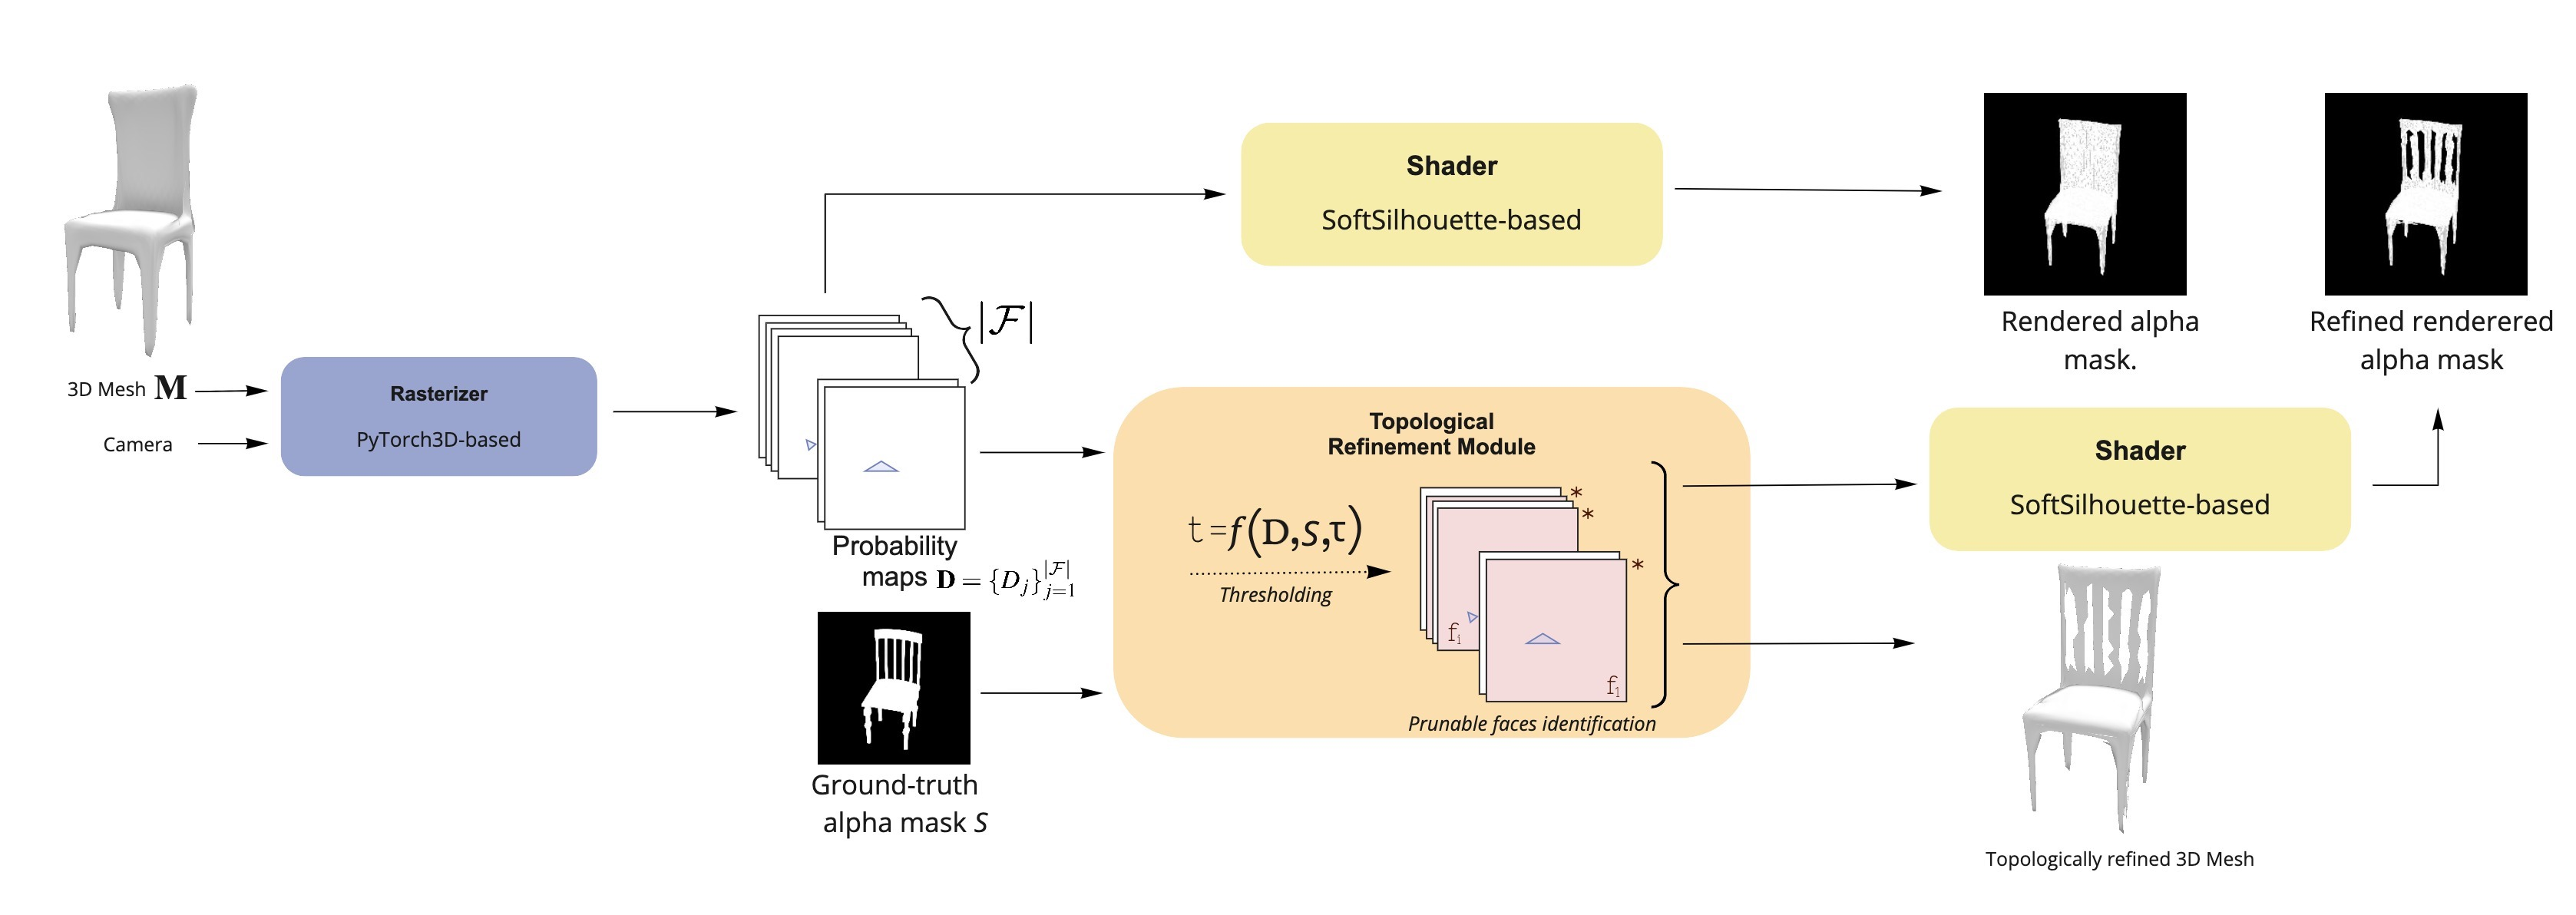
\includegraphics[width=\linewidth]{images/adaptativesr/final_figure.jpg}
\end{center}
    \caption{\textbf{Architecture overview of our method.} Based on a 3D mesh \textbf{M} and a camera pose information, our module leverages onto PyTorch3D rasterizer to detect and prune onto the mesh surface by solely relying on the ground-truth silhouette mask \textit{S}.}
\label{fig:pipeline_overview}
\end{figure*}

Detecting these faces can be accomplished by computing an \ac{IoU} score between the face from $F$ involved in \textbf{M} rendering and the ground-truth mask \textit{S}. These faces can then be removed from the 3D mesh surface or directly discarded in the shader stage of the renderer. Inspired by the thresholding strategy introduced in \citep{pan2019deep}, we establish an adaptative threshold $\tau$ based on the \ac{IoU} score distribution and quantile $Q_{\tau}$:

\begin{equation}
    \tau=Q_{\tau}({\gamma/\Gamma})
\end{equation}

with ${\gamma/\Gamma}$ the \ac{IoU} distribution score and $\tau \in [0,1]$. Similar to the thresholding strategy employed by \citep{pan2019deep}, the value of $\tau$ directly influences the number of pruned faces: the smaller $\tau$ is, the smaller the number of faces detected as incorrectly projected will be.

\subsection{Topological refinement}
We implement our topological refinement strategy using the renderer from PyTorch3D \citep{ravi2020accelarating}. Its modularity is particularly valuable, as it allows the entire rendering process to be  be adjusted as needed. In our work, we  focused on the rasterization stage due to its similarity with the one from SoftRasterizer \citep{liu2019soft}. 

A key difference between SoftRasterizer and PyTorch3D silhouette rasterization process lies in the number of faces considered: PyTorch3D only accounts for the top-\textit{K} closest faces from the camera center of \textbf{M} at each pixel location $p_i$. SoftRasterizer rather equally considers all the faces. 
We denote by $\mathbf{P}\in \mathbb{R}^{K \times H \times W}$ the intermediate probability map generated by \citep{ravi2020accelarating}, which closely relates to the one originally introduced in \citep{liu2019soft}. For any 2D pixel location $p_{i}$ and the $k^{th}$ closest face $f_{k}^{i}$, the distance based probability tensor $\mathbf{P}$ is expressed as follows:

\begin{equation}
    \mathbf{P}[k,p_{i}]=\left(1+e^{-d(f_{k}^{i},p_{i})/\sigma}\right)^{-1} 
\end{equation}

where $d(f_{k}^{i},p_{i})$ stands for the Euclidean distance between $p_i$ and $f_{k}^{i}$. Term $\sigma$ is a hyperparameter that controls the sharpness of the rendered silhouette image. Both $d$ and $\sigma$ were originally defined in SoftRasterizer \citep{liu2019soft}. \newline

We adopt the same soft silhouette shader stage introduced in SoftRasterizer to generate the soft silhouette mask $\hat{S}$ from $\mathbf{P}$ through the aggregation function:

\begin{equation}
    \hat{S}[p_i]=1 - \prod_{k=1}^{K} (1 - \mathbf{P}[k,p_{i}])
\end{equation}

We introduced $\mathcal{F}$ as the set of unique faces involved in the rendering of any mesh $\mathbf{M}$ derived from $\mathbf{P}$. The larger $K$ is, the more likely the cardinality of $\mathcal{F}$ will get closer to the total number of faces in the original mesh $|F|$. 

Finally, since $\mathbf{P}$ is structured differently from SoftRasterizer, we denote $\mathbf{D}=\{D_{j}\}_{j=1}^{|\mathcal{F}|}\in \mathbb{R}^{|\mathcal{F}|\times H\times W}$  as the equivalent probability map tensor as defined in SoftRasterizer \citep{liu2019soft}.

Our module determines whether a face should be pruned based on the degree of overlap between the ground truth mask $S$ and the rendered face. Since each face $f_{j} \in \mathcal{F}$ contributes to the final rendered silhouette through its probability map $D_{j}\in \mathbb{R}^{H\times W}$, the \ac{IoU} term $\gamma_{j}/\Gamma_{j}$ is computed: 

\begin{equation}
\begin{cases}
     \gamma_{j}=\sum_{p_{i}\in S} \min \left(  D_{j}[p_{i}] , S[p_{i}] \right) \\
     \Gamma_{j}=\sum_{p_{i}\in S} \max \left( D_{j}[p_{i}],S[p_{i}] \right)
\end{cases}
\end{equation}

We extend the computation from a single face $f_{j}$ to all the faces in $\mathcal{F}$, and denote $\gamma/\Gamma \in \mathbb{R}^{|\mathcal{F}|}$ the complete \ac{IoU} score distribution.

Our method then leverages this distribution to identify which faces should be pruned from $\mathbf{M}$. We implement a thresholding strategy partially inspired by \citep{pan2019deep}, where an adaptive threshold $t$ is set based on statistical quantile considerations. Faces with an \ac{IoU} score lower than $t=Q_{\tau}(\gamma/\Gamma)$ are pruned from $\mathbf{M}$. This approach allows for dynamic adaptation of the number of faces to prune. 

\section{Experiments}
\label{sec:experiments}

\textbf{Dataset.} Our approach has been extensively tested using ShapeNetCore \citep{chang2015shapenet}. In line with the TMN \citep{pan2019deep}, our experiments focus on the topologically challenging \textit{Chair} class from ShapeNet \citep{chang2015shapenet}. It contains a total of 6,774 different chairs, with 1,356 instances in the test set.

\noindent\textbf{Metrics.} For 2D evaluation, we use the 2D \ac{IoU} to measure how well the refined mesh produced by AdaptativeSR aligns with the ground truth mask, compared to the non-refined mesh. For 3D evaluation, the \ac{CD}, F-Score and METRO distance are considered. The METRO criterion, first introduced in \citep{cignoni1998metro} and reconsidered in AtlasNet \citep{groueix2018papier} work, is motivated by its ability to consider mesh connectivity, unlike the \ac{CD} or F-score metrics, which only focus on 3D point clouds distribution. 

\noindent\textbf{3D Mesh generation network.} Our refinement module is compatible with any image-based 3D reconstruction pipeline, making it agnostic to the network responsible for producing the 3D mesh. We chose to work with meshes generated by TMN \citep{pan2019deep}. Since our focus is extensively on face-pruning, we only trained the ResNet18 encoder with the first stage of their 3D mesh reconstruction architecture, referred to as \textit{SubNet-1} in \citep{pan2019deep}, and abbreviated it as TMN in this section. The TMN architecture includes a deformation network and a learned topological modification module. It's worth noting that the TMN architecture \citep{pan2019deep} was trained and used for inference with 3D ground truth labels and sources images from 3D-R2N2 \citep{choy20163d}. We refer to the deformation network preceding the topology modification network \citep{pan2019deep} as the \textit{Baseline}. The $genus-0$ 3D mesh produced by the \textit{Baseline} network is derived from a 3D sphere template with 2562 vertices.

\noindent\textbf{PyTorch3D Renderer.} We use the PyTorch3D \citep{nie2020total3dunderstanding} differentiable renderer, setting $K=30$ and $\sigma=5.10^{-7}$ to produce the sharpest binary alpha masks. All the silhouette masks used in this section were generated with the PyTorch3D renderer as have a $224\times 224$ resolution. Similar to the rendering approach used in \citep{choy20163d,liu2019soft,yan2016perspective}, we rendered 24 views per mesh with a fixed camera distance $d_{camera}=2.732m$ and an elevation angle of $30\degree$. The azimuth angle varied by an increment of $15\degree$ from $0\degree$ to $345\degree$. All the meshes predicted by \citep{pan2019deep} were normalised in the same way as those in ShapeNetCore \citep{chang2015shapenet}. 

We demonstrate the effectiveness of our method by relying solely on 2D binary masks and the modularity of the renderer. 

\subsection{Topological refinement evaluation - Qualitative results}

Our main objective is to demonstrate how accurately we can detect the relevant faces on the 3D mesh that should be pruned during rendering. Figure \ref{fig:face2prune} highlights the faces identified as poorly rendered compared to the ground-truth silhouette mask on three different chairs. Based on these 2D silhouette considerations, our method achieves visually more appealing results than \citep{pan2019deep}. 

\begin{figure*}[htp!]%[htp!]
\begin{center}
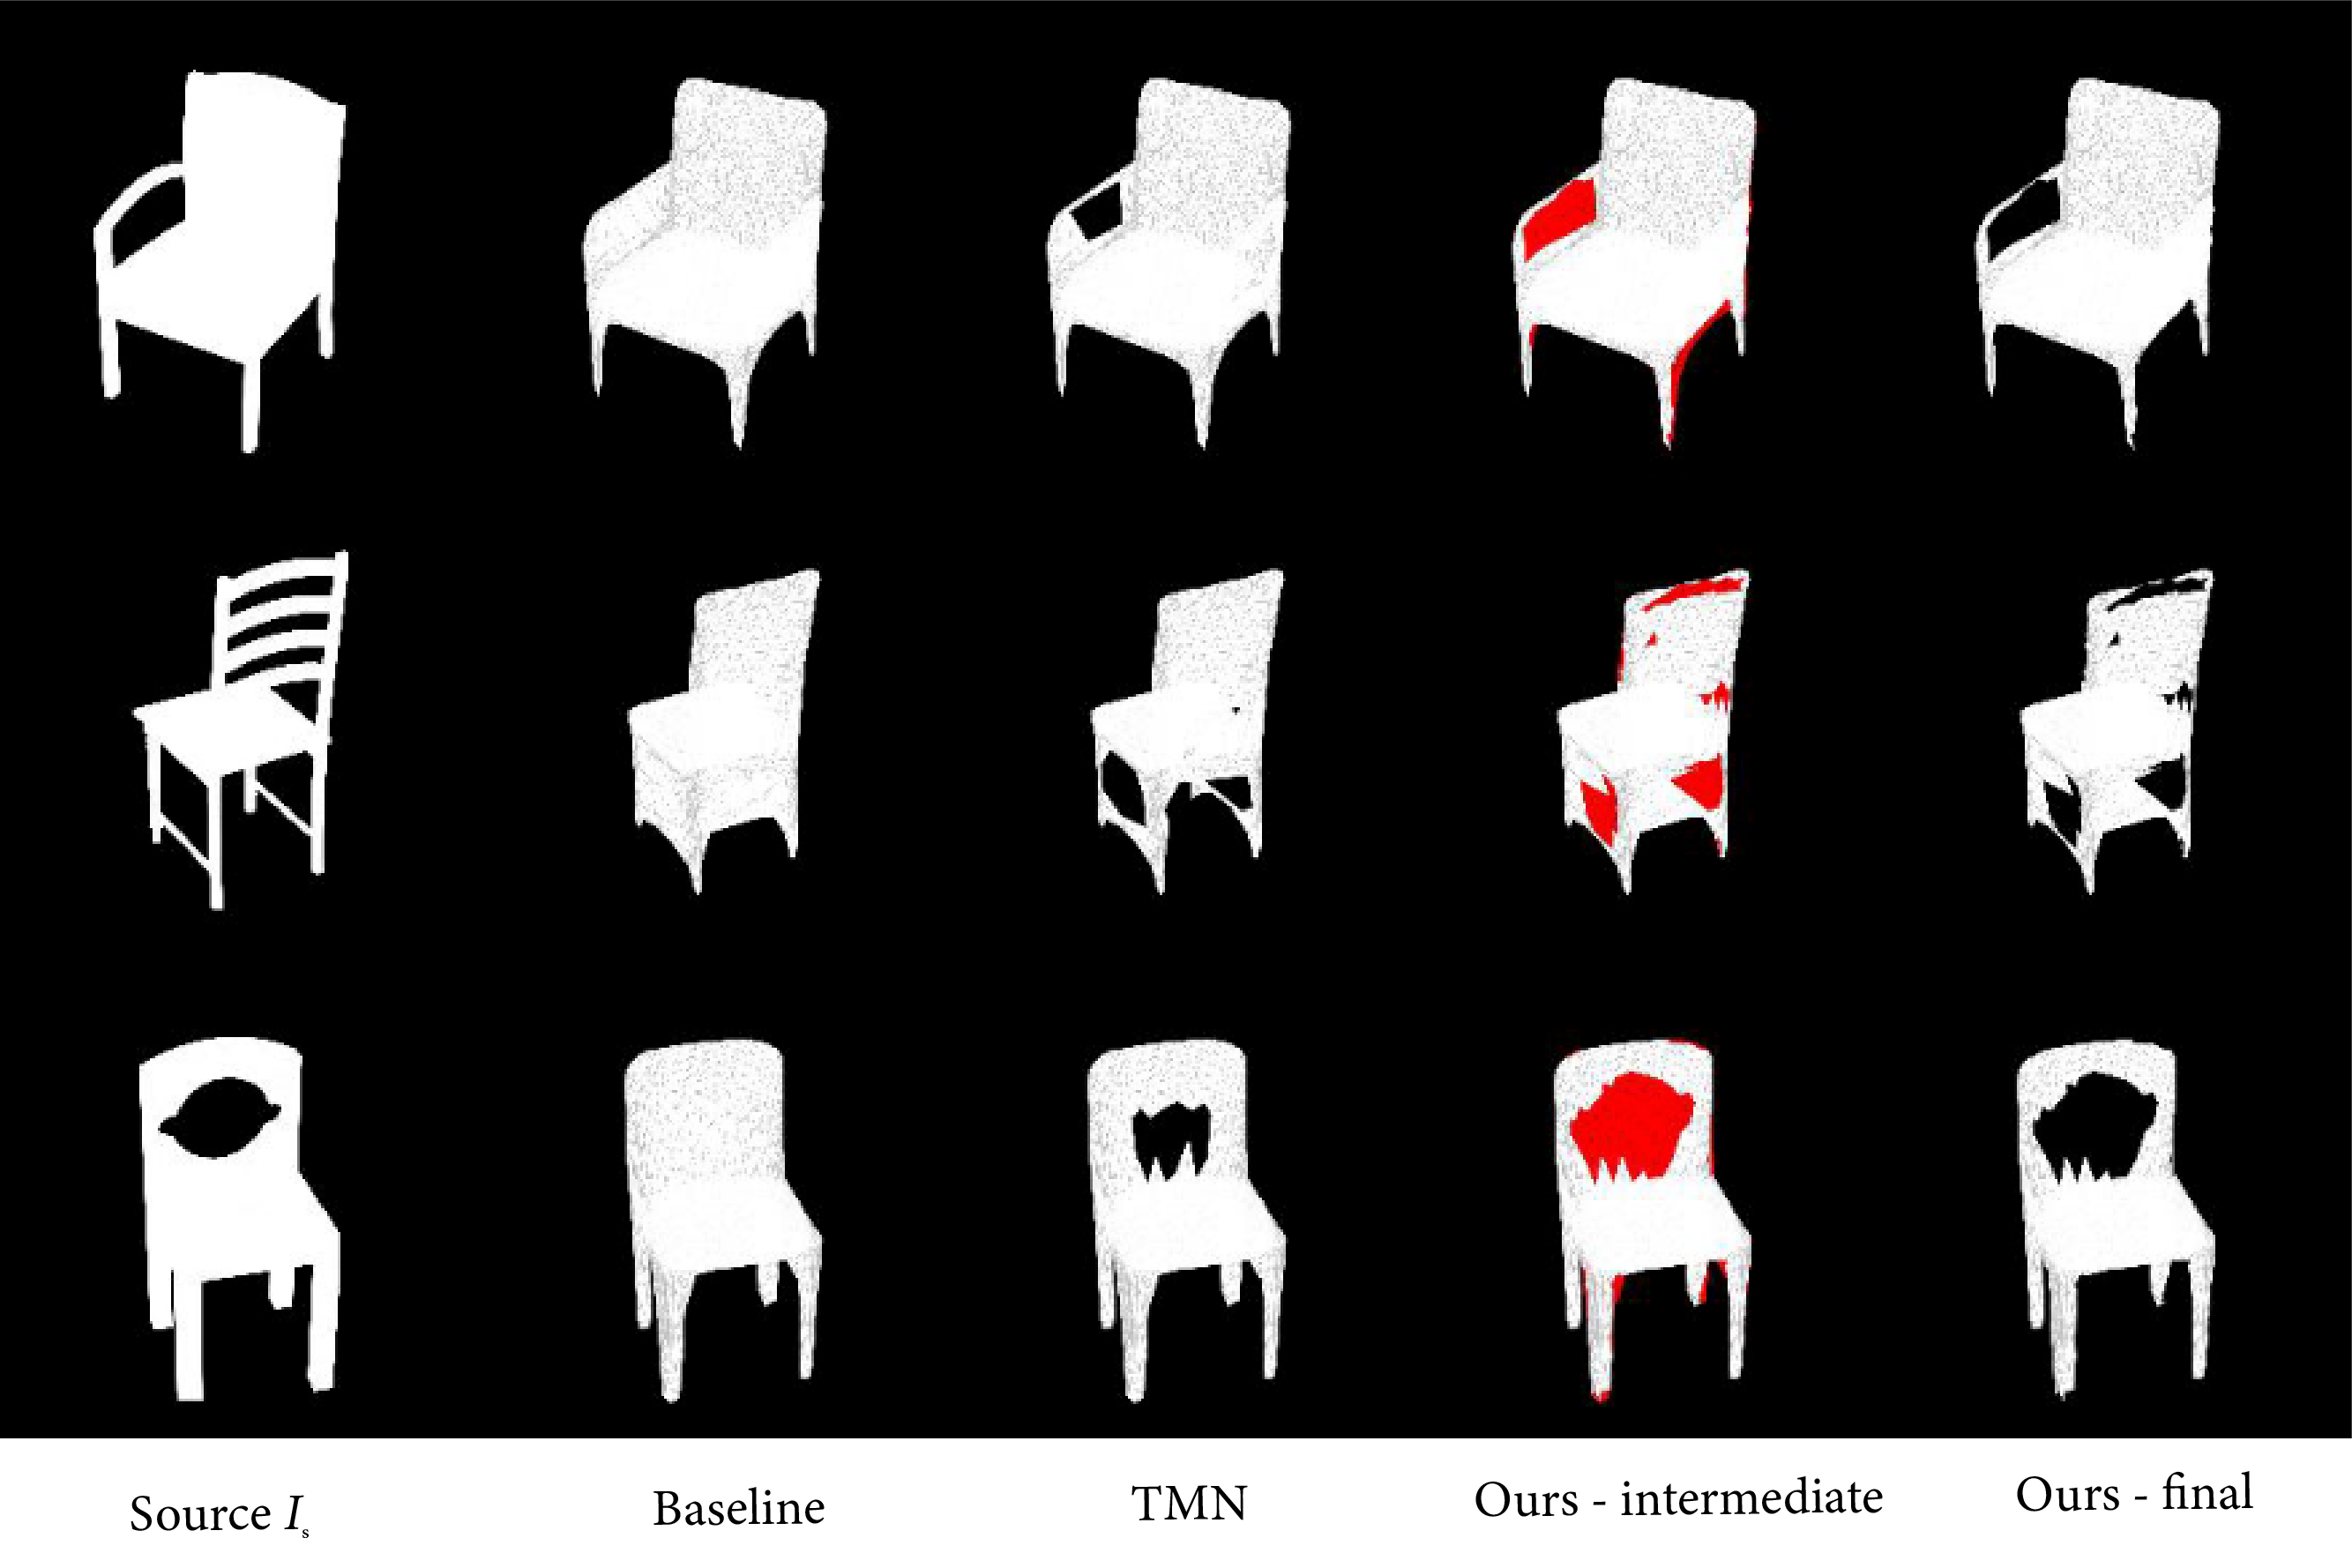
\includegraphics[width=\linewidth]{images/adaptativesr/highlight_faces_New.png}
\end{center}
    \caption{\textbf{Silhouette based comparison on several instance from the ShapeNetCore test set.} Faces rendered onto red regions in our results (called \textit{intermediate}) should be pruned on 3D mesh surface. Our final renderings are shown on the last column. We fixed $\tau = 0.05$.}
\label{fig:face2prune}
\end{figure*}

Figure \ref{fig:pruning_multi_view} further illustrates this observation from six different viewpoints of the same chair. In this specific example, the TMN pruning module failed to identify faces that should be pruned, resulting in an unchanged mesh compared to the \textit{Baseline}. In contrast, our method effectively pruned the faces that were rendered the least accurately, as determined by the ground truth alpha mask. The faces pruned in each view are independent each others. 

\begin{figure*}[htp!]%[htp!]
\begin{center}
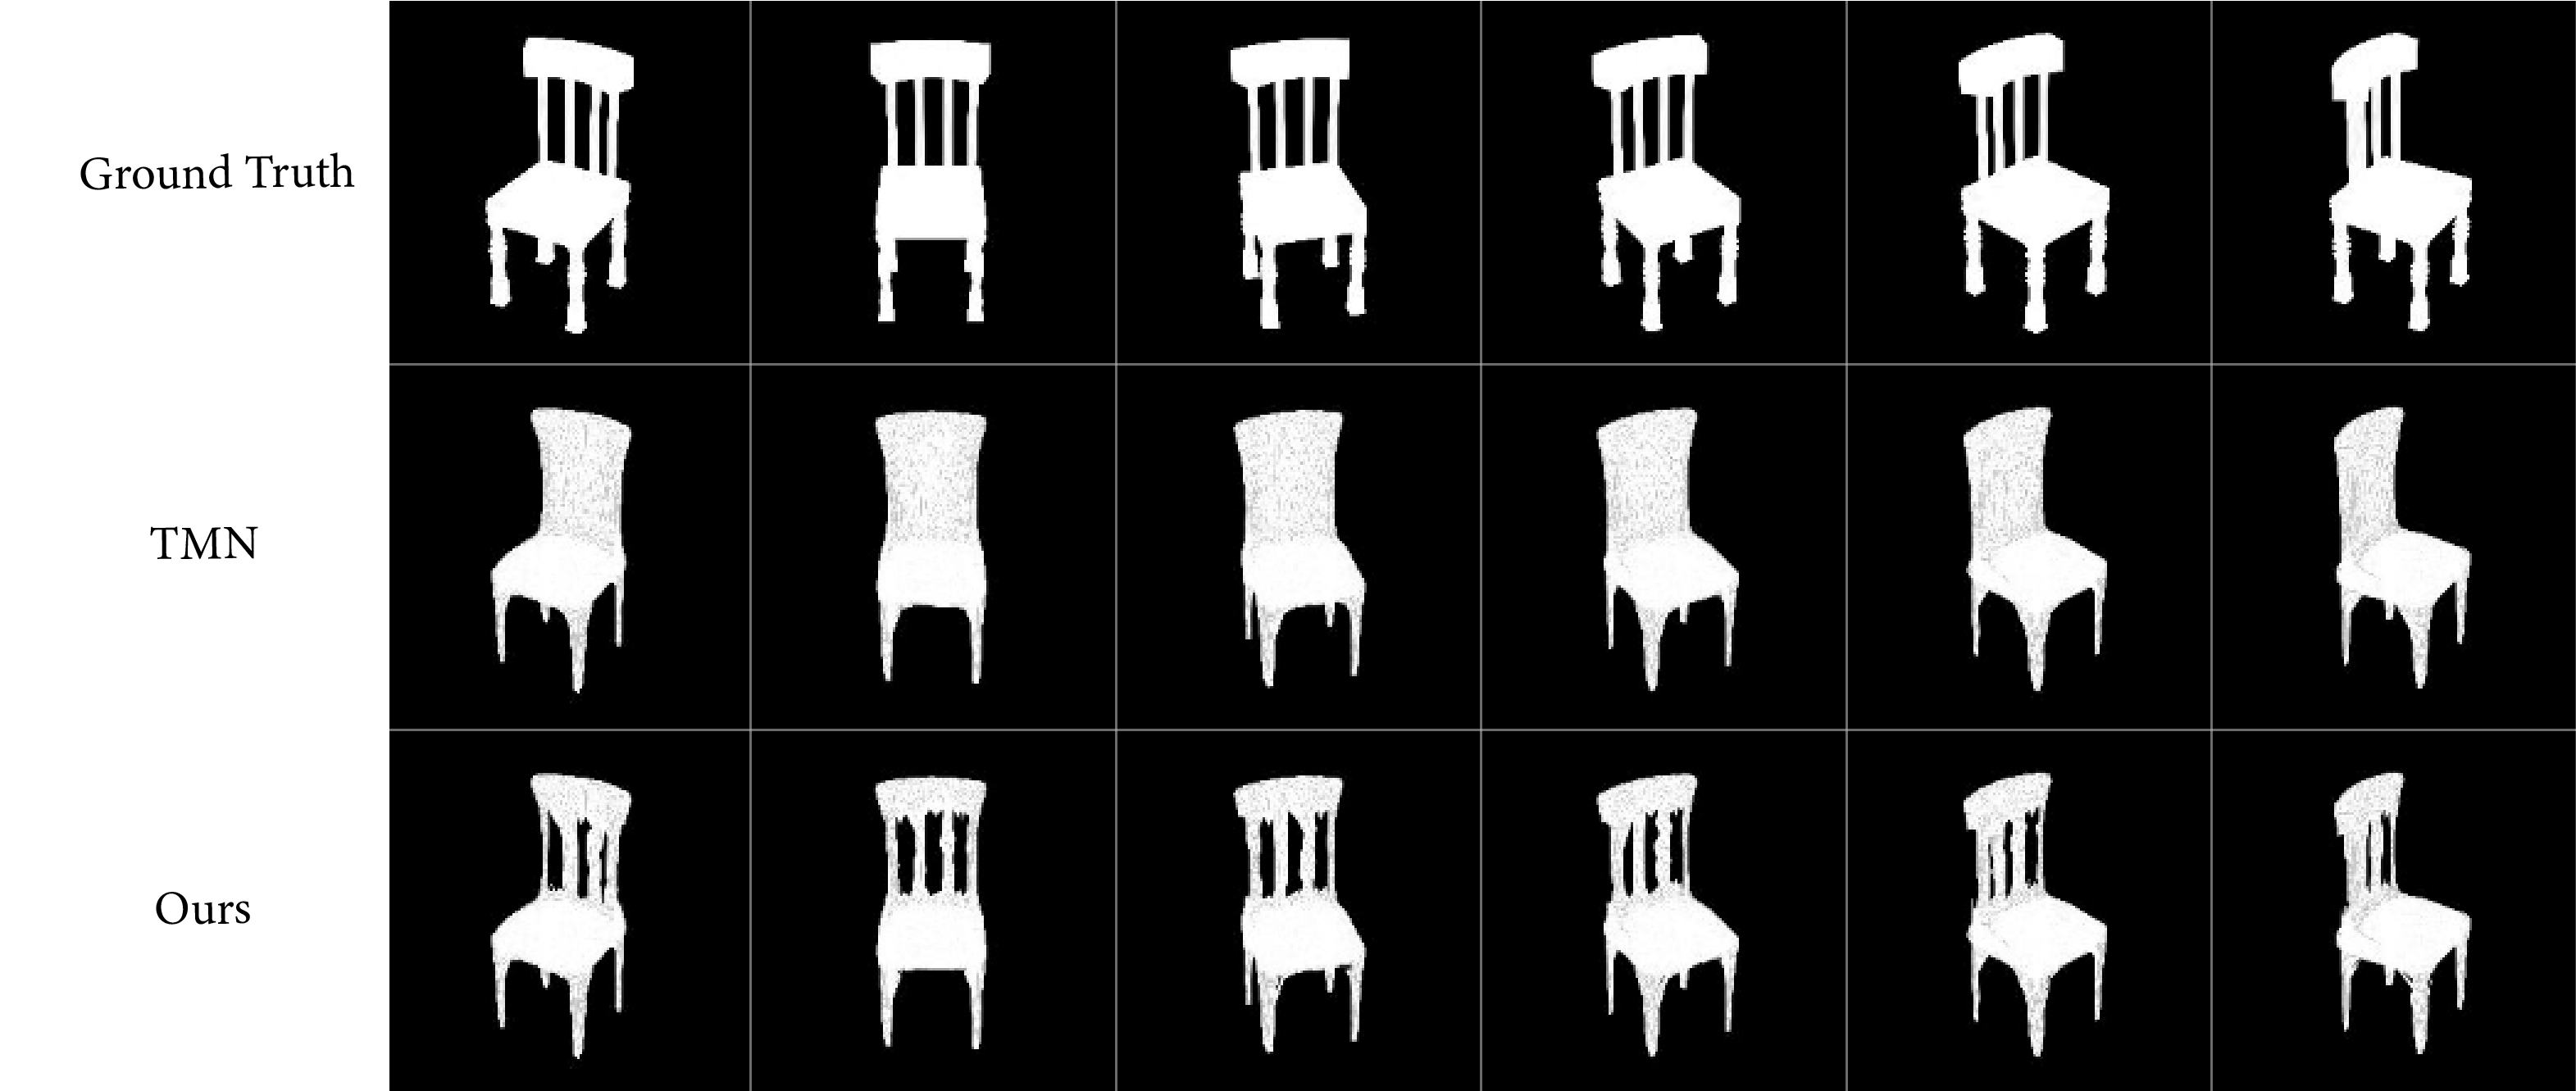
\includegraphics[width=\linewidth]{images/adaptativesr/severalview2D_New.png}
\end{center}
    \caption{\textbf{Rendered silhouette mask results on 6 viewpoints}. Whereas TMN \citep{pan2019deep} may fail to accurately update the mesh topology in these cases, our method prune relevant faces. We fixed $\tau = $ \textbf{0.05}.}
\label{fig:pruning_multi_view}
\end{figure*}

The viewpoint associated with a challenging azimuth angle in the last column of Figure \ref{fig:pruning_multi_view} still provides sufficient information for our AdaptativeSR module to remove the relevant faces during rendering.

\subsection{2D and 3D-based quantitative evaluation} 

We compare performances of our method using different thresholds $\tau$ in Table \ref{tab:sota_table}, along with the meshes produced by both the \textit{Baseline} network and TMN \citep{pan2019deep}. From the 1,356 inferred meshes in the ShapeNetCore\citep{chang2015shapenet} test set, we manually selected 50 highly challenging meshes (from a topological perspective) and rendered them using the 24 different camera viewpoints described earlier. The threshold associated with the F-score was set to 0.001. A total of 10,000 points were uniformly sampled across the surfaces of the different meshes to compute these 3D metrics. 

\begin{table}[htp!]
    \caption{\textbf{2D and 3D-based metric scores comparison with the Baseline and TMN} \citep{pan2019deep} - Presented results were averaged over the 50 instance from our manually curated test set and over the 24 different viewpoints for the 3D metrics. Best results are highlighted in \colorbox{red!25}{red}, second best in \colorbox{orange!25}{orange} and third ones in \colorbox{yellow!25}{yellow}.}
    \label{tab:sota_table}
    \begin{center}
    \centering
    \begin{adjustbox}{width=\textwidth}
    \begin{tabular}[h]{c||cccc}
    \hline
    Method \textit{(2D/3D supervision)} &  2D IoU ($\uparrow$) & CD ($\downarrow$) & F-Score ($\uparrow$) & METRO ($\downarrow$) \\[.5pt]
    \hline
    \textit{Baseline} (-)& 0.660  &  6.602  & 53.27  &  1.419  \\[1.5pt]
    TMN \citep{pan2019deep} (3D)  & 0.681  & \cellcolor{red!25}{6.328}   & \cellcolor{red!25}{54.23}  & \cellcolor{red!25}{1.293} \\
    \hline 
    Ours $\scriptstyle \tau=0.01$ (2D) & 0.747 &\cellcolor{yellow!25}{6.541}  &  \cellcolor{orange!25}{53.39} &  1.418      \\
    Ours $\scriptstyle \tau=0.03$ (2D) & 0.755 &6.539  & \cellcolor{orange!25}{53.39}  &    \cellcolor{yellow!25}{1.417}  \\
    Ours $\scriptstyle \tau=0.05$ (2D) & \cellcolor{yellow!25}{0.763} & \cellcolor{orange!25}{6.540}  &  \cellcolor{yellow!25}{53.34} &   \cellcolor{yellow!25}{1.417}     \\
    Ours $\scriptstyle \tau=0.1$ (2D)& \cellcolor{red!25}{0.778} & 6.551  & 53.27 &  \cellcolor{orange!25}{1.416}     \\
    Ours $\scriptstyle \tau=0.15$ (2D)& \cellcolor{orange!25}{0.771} & 6.548  & 53.26  &    \cellcolor{orange!25}{1.416}   \\
    \hline 
    \end{tabular}
    \end{adjustbox}
    \end{center}
    
    \end{table}

AdaptativeSR outperforms the learned topology modification network from TMN \citep{pan2019deep} based on the 2D \ac{IoU} scores, as shown in Table \ref{tab:sota_table}. The results presented for TMN \citep{pan2019deep} are derived solely from the initial learned topological modification network and do not take into account the topological refinement made by \textit{SubNet-2} and \textit{SubNet-3} networks. Although none of our configurations achieved better scores on the 3D metrics than TMN \citep{pan2019deep}, we emphasize on two key points: \begin{enumerate}
    \item The topologically refined meshed produced by AdaptativeSR consistently outperform those generated by the \textit{Baseline} network.  
    \item Our face-pruning strategy relies only on a unique 2D silhouette mask and does not require any form of 3D supervision, in contrast to \citep{pan2019deep}. 
\end{enumerate}

Since AdaptativeSR has a 2D-based pruning methodology, the evaluation metrics are dependent from the camera viewpoint we choose for performing the topological refinement. Figure \ref{fig:pruning_viewpoint_influence} illustrates the extent to which the camera pose affects both the 2D \ac{IoU} and the \ac{CD} scores.

\begin{figure}[h!]
  \centering
  \subfloat[a][2D IoU]{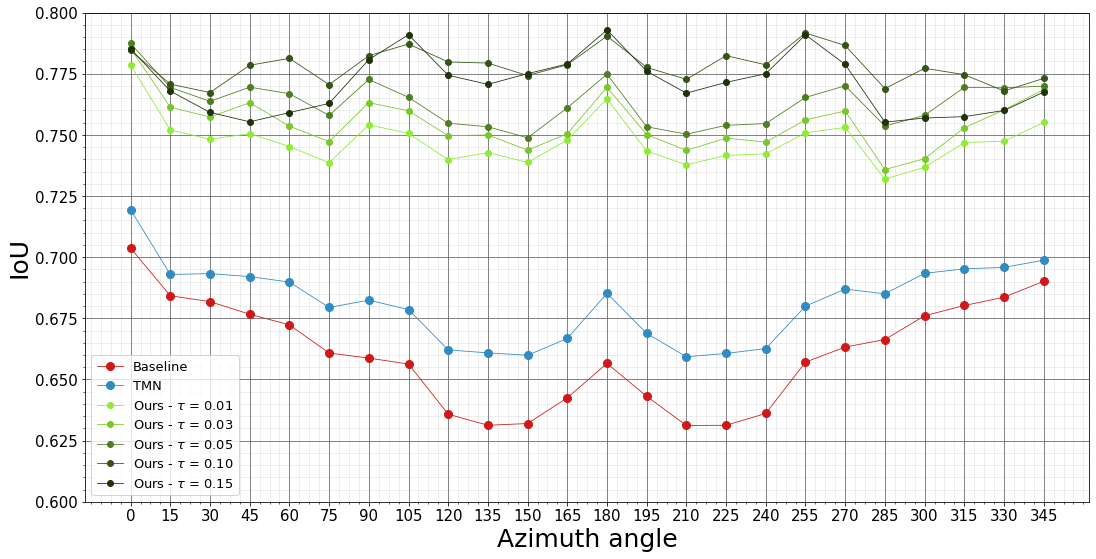
\includegraphics[width=\linewidth]{images/adaptativesr/multiviewsPLOT.png} \label{fig:a}} \\
  \subfloat[b][Chamfer distance]{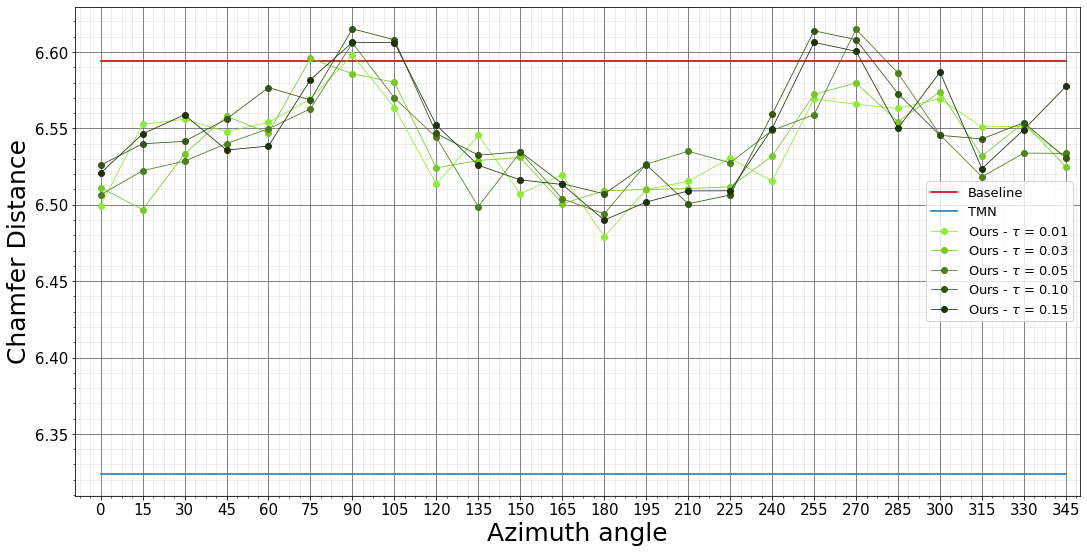
\includegraphics[width=\linewidth]{images/adaptativesr/plot_Chamfer_Distance_last.png} \label{fig:b}}
  \caption{\textbf{Camera viewpoint performances influence} AdaptativeSR is a view-dependant method that fails to consistently prune faces from any viewpoint with the same accuracy.} 
  \label{fig:pruning_viewpoint_influence}
\end{figure}

Azimuth angles around the symmetrical pair $\{90^{\degree}, 270^{\degree}\}$ present more challenges, as there are not as informative as the $180^{\degree}$ viewpoint. Indeed, AdaptativeSR struggles to outperform the \textit{Baseline} architecture in these cases. Our test set is slightly imbalanced, containing only a few chair instances with armrests that require topological refinement, while there is a greater number of instances with topologically complex back structures. Consequently, our method performs slightly worse than the \textit{Baseline} around $90^{\degree}$ and $270^{\degree}$ angles, as the intricate back structures of the chairs are not visible from these viewpoints. 

We also quantitatively confirm on Figure \ref{fig:pruning_viewpoint_influence} the anticipated impact of $\tau$ during the rendering process on the 2D \ac{IoU} score: the higher $\tau$ is set, the more faces we discard. 

\section{Limitations and further work}

Our method demonstrates encouraging results in refining the topology of 3D meshes through 2D silhouette mask considerations, even though it has a few remaining limitations. First, the thresholding strategy we use to determine whether a face should be pruned from the 3D mesh surface requires to set a fixed hyperparameter $\tau$, and thus some empirical experiments. We align with \citep{nie2020total3dunderstanding} regaring the need to rely on local 2D and 3D prior information to build a more robust thresholding strategy. Additionally, AdaptativeSR may exhibit incorrect behaviour with faces that are rendered close to the silhouette boundary edges. 

From a broaderer perspective, our method currently relies on 2D masks and thus overlooks texture information from RGB images. While impressive 3D textured results have been achieved using UV mapping in self-supervised image-based 3D reconstruction methods with genus-0 meshes \citep{li2020self,pavllo2020convolutional}, to the best of our knowledge, no attempts have been made to advance beyond such first-order representations. Finally, since our work is agnostic to the 3D mesh reconstruction network, a natural next step would be to design a complete self-supervised 3D reconstruction pipeline that incorporates AdapativeSR. 

\section{Conclusion}
\label{sec:conclusion}
We proposed a novel approach for performing topological refinement on 3D meshes surfaces by exclusively considering 2D alpha masks and leveraging the modularity of the PyTorch3D rasterization framework. To the best of our knowledge, no prior attempts in our line of work were made in 2019/2020, as both TMN \citep{pan2019deep} and Total3D \citep{nie2020total3dunderstanding} rely on 3D-supervised neural networks for pruning faces and edges. The agnostic design of AdaptativeSR allows any self-supervised image-based 3D reconstruction pipeline (built with the PyTorch3D framework) to leverage the advancements we presented for reconstructing topologically complex meshes. We achieved consistent and competitive results from a topological perspective when compared to the 3D-based pruning strategy from TMN \citep{pan2019deep}. 

\chapter{EpipolarNVS: Additional ressources}
\label{annex:epipolarnvs}

We provide some additional information regarding the Chapter ~\ref{chapter:epipolarnvs}. 

\section{Dataset characteristics}
\label{annex:epipolarnvs-dataset}

We decided not to use the same ShapeNet dataset version as \citep{kim2020novel, sun2018multiview} used in their work. We worked with the rendered ShapeNet images from DISN \citep{xu2019disn}. This dataset offers at least three main improvements over the one used in \citep{kim2020noveln,sun2018multiview}:

\begin{itemize}
    \item Intrinsic camera parameters are available. 
    \item Each object within a class has 36 different views (against 18 for the dataset provided by \cite{kim2020novel,sun2018multiview}). 
    \item The rendered images have a non-zero elevation angle, and the azimuth angle is sampled on a regular 10° basis. A random noise term is added to each rendered view to slightly jitter the camera pose. 
\end{itemize}

Considering real-world Synthia \citep{ros2016synthia} and KITTI \citep{geiger2012we} datasets, the original data used in \citep{kim2020novel} only contain extrinsic matrices, leaving aside the intrinsic information required by our architecture. We therefore built our own train/test sets using the same scenes as \citep{kim2020novel}. The images were resized to $256\times256$ for speed purposes, and the ground-truth intrinsic matrices were adjusted accordingly. The images in these real-world scenarios are more challenging than those in \citep{kim2020novel,sun2018multiview} since dealing with center-cropped images eliminates fast-moving elements (at the image borders) from the scenes.

Finally, we follow the same setting as in \citep{kim2020novel} for the maximum latitude between the source and target views: a full $\pm 180^{\circ}$ azimuthal range is allowed for the ShapeNet classes, while a maximum of $\pm 10$ frames is considered for the real world datasets Synthia \citep{ros2016synthia} and KITTI \citep{geiger2012we}.

\section{Additional results}

Additional qualitative results from our EpipolarNVS model across the four datasets are presented below. For each dataset, we showcase 8 different scenes or object instances.

\begin{figure*}[htp!]
    \begin{center}
    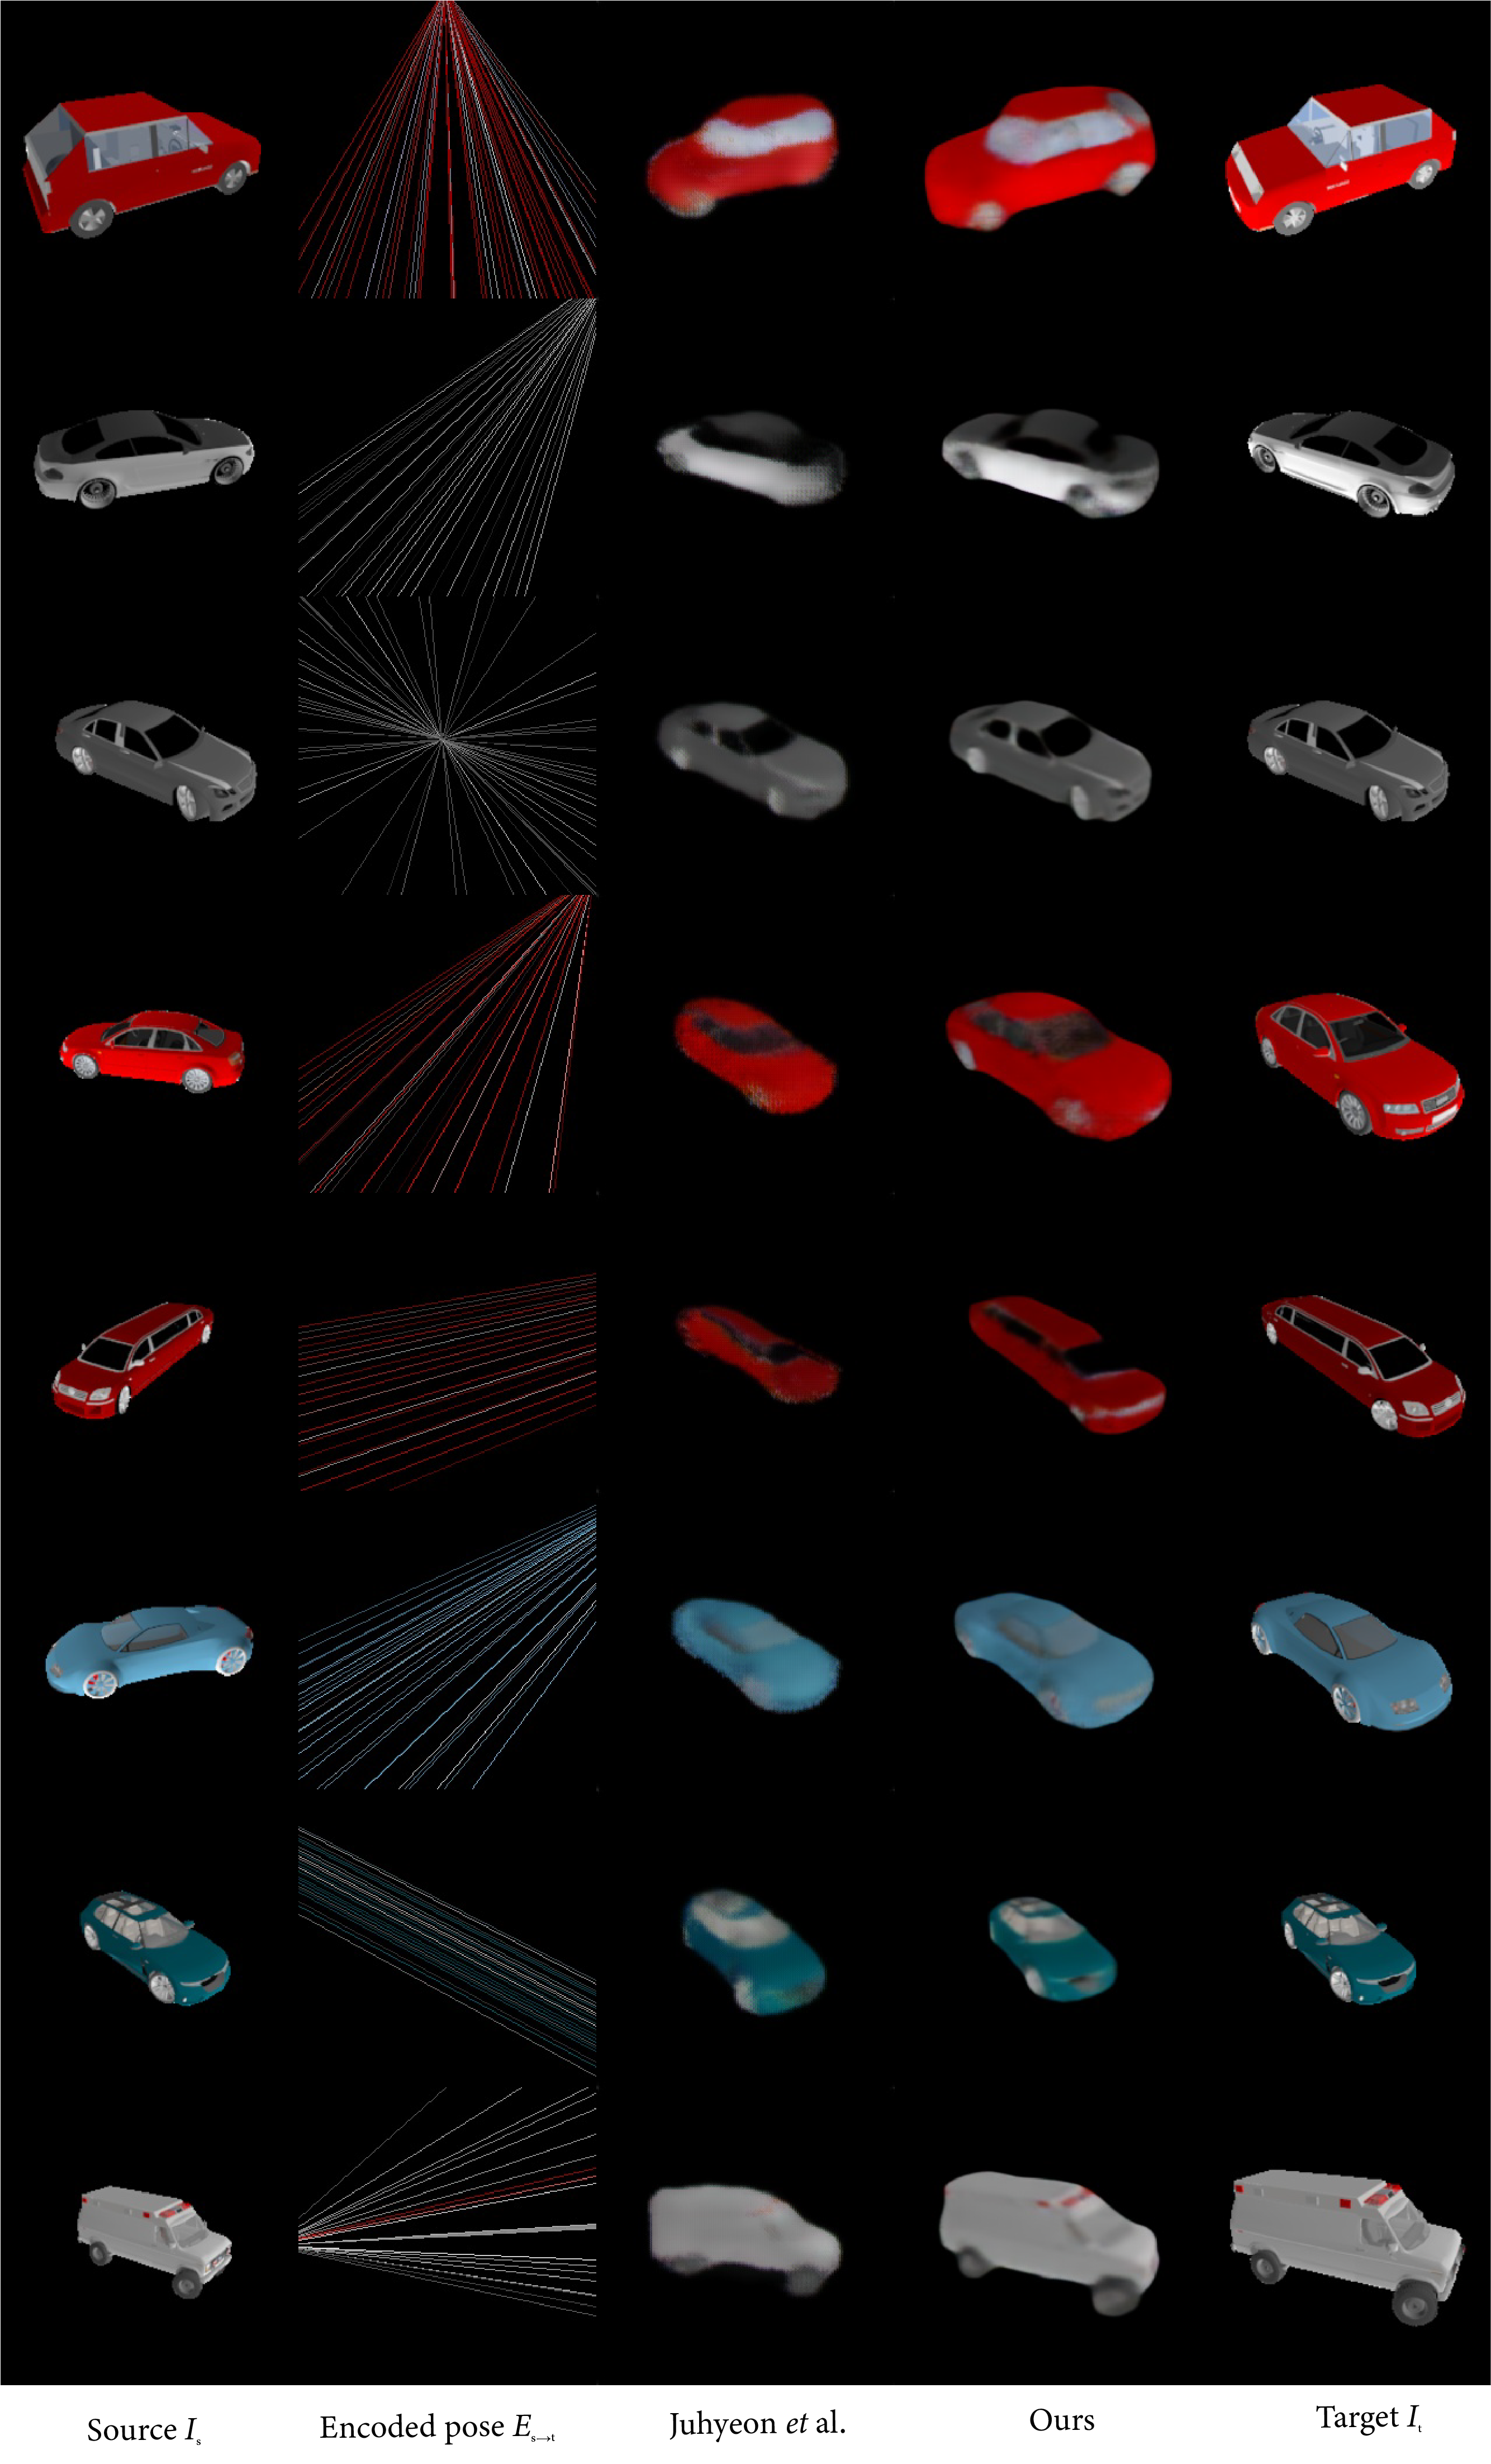
\includegraphics[width=0.95\textwidth]{images/epipolarnvs/SuppMat_Car_New.png}
    \end{center}
     \caption{\textbf{Visual results from the test ShapeNet} \citep{xu2019disn} \textit{Car} \textbf{class}.}     
     \label{fig:add_visCar}
\end{figure*}

\begin{figure*}[htp!]
    \begin{center}
    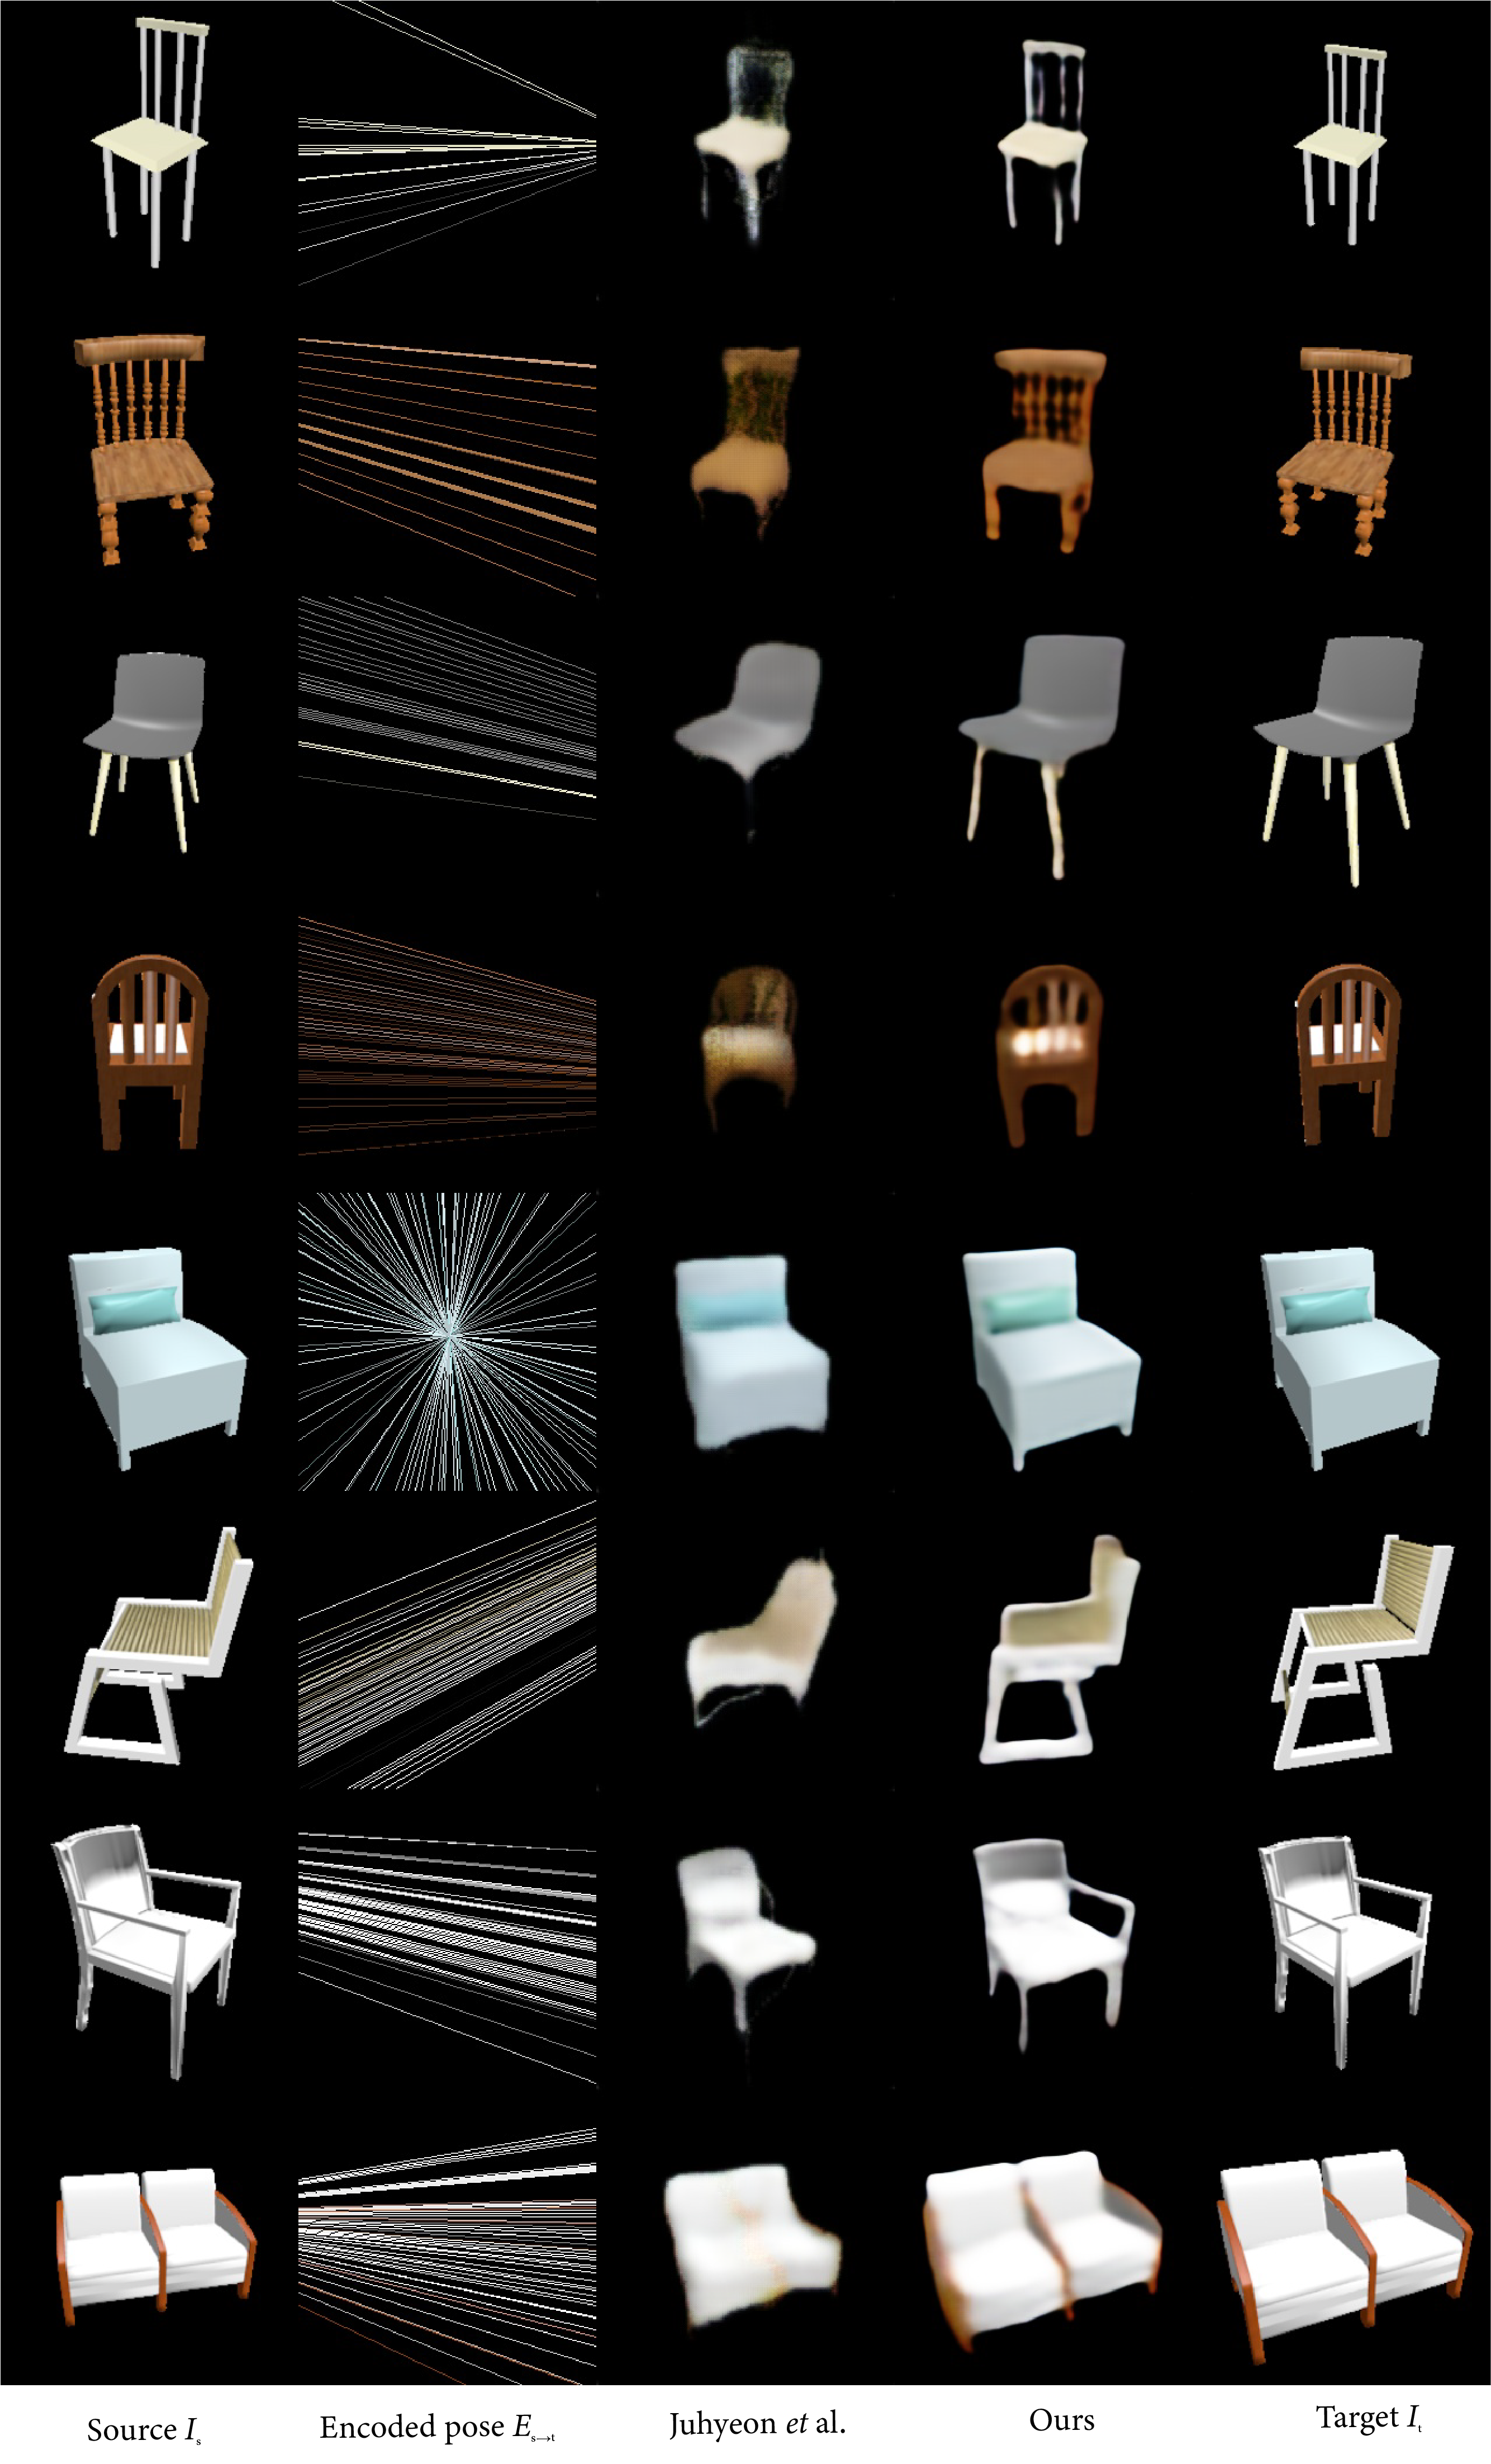
\includegraphics[width=.95\textwidth]{images/epipolarnvs/SuppMat_Chair_New.png}
    \end{center}
     \caption{\textbf{Visual results from the test ShapeNet} \citep{xu2019disn} \textit{Chair} \textbf{class}.}
     \label{fig:add_visChair}
\end{figure*}

\begin{figure*}[htp!]
    \begin{center}
    \includegraphics[width=.95\textwidth]{images/epipolarnvs/SuppMat_Synthia_New.png}
    \end{center}
     \caption{\textbf{Visual results from Synthia} \citep{ros2016synthia}.}
     \label{fig:add_visSynthia}
\end{figure*}

\begin{figure*}[htp!]
    \begin{center}
    \includegraphics[width=.95\textwidth]{images/epipolarnvs/SuppMat_KITTI_New.png}
    \end{center}
     \caption{\textbf{Visual results from KITTI} \citep{geiger2012we}.}
     \label{fig:add_visKITTI}
\end{figure*}

\chapter{EpiNeRF: Additional ressources}

Further details about Chapter ~\ref{chapter:epinerf}, including EpiNeRF internal structure, training process, and view synthesis performance, are presented here. 

\section{EpiNeRF submodules and training}

\subsection{Feature radiance fields: NeRFeature $\Psi$}

NeRFeature's internal architecture is illustrated in Figure \ref{fig:supp_nerfeature}. It closely mirrors the radiance structure of $\Phi$, even though there is no hypernetwork to predict its weights. NeRFeature is designed to produce deep features that lie in the latent space learned by $\chi$, similar to the approach implemented by \citep{ye2023featurenerf} through its distillation of foundation models \citep{oquab2023dinov2}. Our feature distillation strategy transfers information from the 2D model $\chi$ into 3D.  

\begin{figure}[htp!]
    \begin{center}
  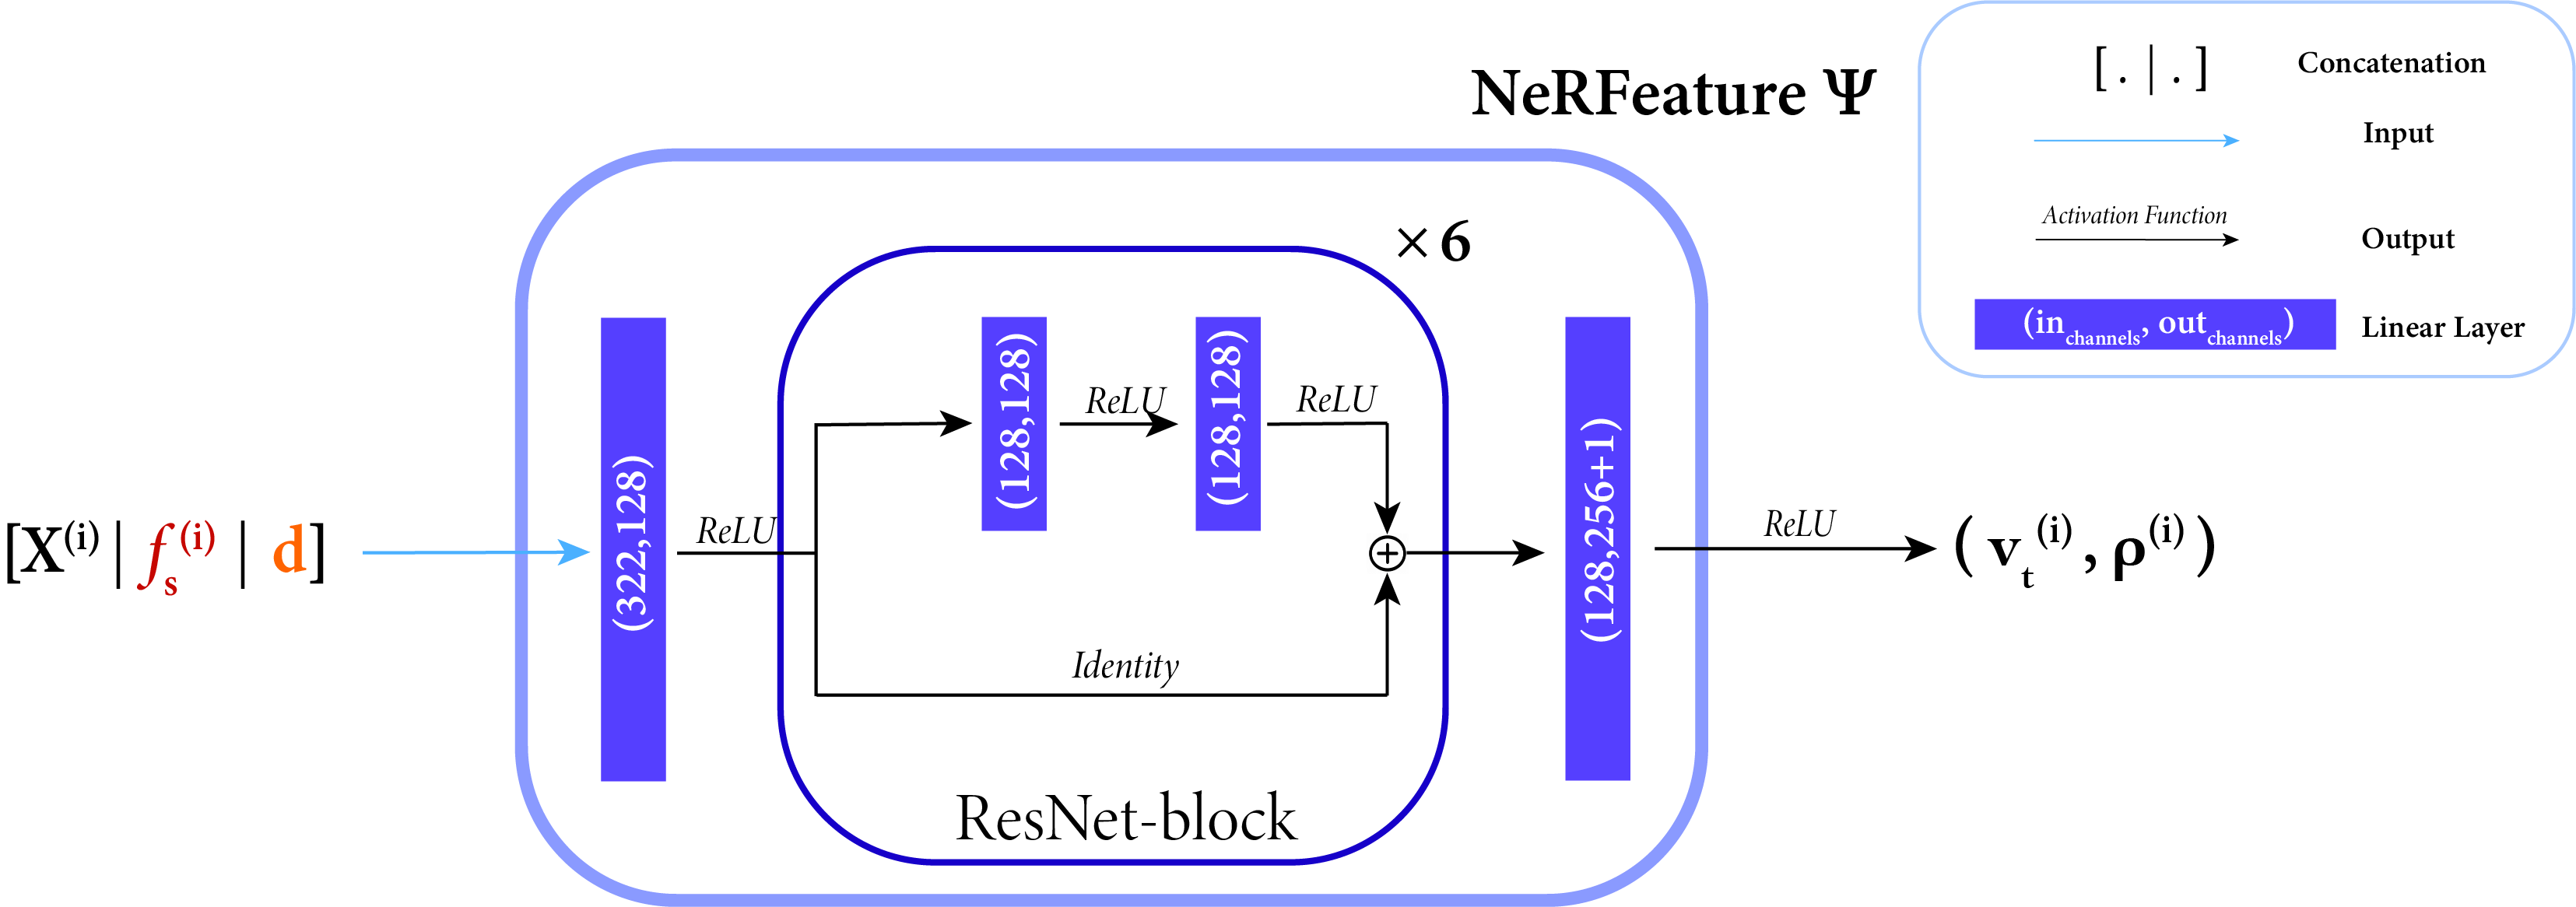
\includegraphics[width=\linewidth]{images/epinerf/supp_nerfeature.png}
  \caption{\textbf{NeRFeature overview.} NeRFeature implements a six ResNet blocks with an extended output that lives in $\mathbb{R}^{d_{\text{feat}}}$. Such an intermediate dense feature, with a transparency scalar, is later involved in the volume rendering operation to get $f_{t}$.}
  \label{fig:supp_nerfeature}
  \end{center}
\end{figure}


We get the final target-aligned deep feature from the derived vanilla volume rendering equation \eqref{eq:main_nerf} :

\begin{equation}
\label{eq:ft_vr}
    f_{t} = \sum_{i=1}^{N_{s}} T^{(i)}(1-exp(-\rho^{(i)}\delta_{i}))\mathbf{v}_{t}^{(i)} \in \mathbb{R}^{d_{\text{feat}}}
\end{equation}
with $T^{(i)} = \exp\left(-\sum_{j=1}^{i-1}\rho^{(j)}\delta_{j}\right)$ the accumulated transmittance along \textbf{r}.

As shown in Figure \ref{fig:supp_nerfeature}, the symmetrical pixel-wise feature $f_{s,symm}^{(i)}$ is not used as input for NeRFeature $\Psi$. Integrating a 3D symmetry prior into a high-dimensional space like $\mathbb{R}^{d_{\text{feat}}}$ is more complex than in RGB space. NeRFeature therefore only receives a 3D point location, a direction, and the source-aligned feature $f_{s}^{(i)}$ as input.

\subsection{Epipolar-based feature attention}
\label{appendix:epinerf-feature}
This section gives additional explanations about our light feature attention mechanism.

As introduced in section \ref{subsec:epipolar_att}, the target-aligned features $f_{t}$ and the source-aligned one $f_{s}^{(i)}$ are used to compute the light cross-attention score $\mathbf{s}_{a}^{(i)}$:

\begin{equation}
    s_{a}^{(i)} = \frac{\mathbf{q}^{T}\mathbf{k}}{\sqrt{d_{\text{feat}}}}= \frac{f_{t}^{T}\times f_{s}^{(i)}}{\sqrt{d_{\text{feat}}}}
\label{eq:attention}
\end{equation}
while $\mathbf{s}_{a}$ denotes the entire distribution over all the points sampled along the ray \textbf{r}.

However, the cross-attention distribution $\mathbf{s}_{a}$ cannot be used directly in the volume rendering equation. The distribution lacks the sharpness needed to effectively influence the volume rendering process. It must be shrunk and normalized around its maxima in a differentiable manner to produce the final distribution $\hat{\mathbf{s}_{a}}$\footnote{Simplified as $\mathbf{s}_{a}$ in the associated chapter for convenience.}.

We thus designed two scaled sigmoid functions, called $S^{k}$ and $S^{K}$ to shrink $\mathbf{s}_{a}$ : 

\begin{equation}
\begin{split}
\hat{\textbf{s}}_{a} &= S^{K}(\textbf{s}_{a})\times S^{k}(\textbf{s}_{a}) \\
S^{q}(\mathbf{s}_{a}) &= \left(1- e^{q(\mathbf{s}_{a}-a_{0})}\right)^{-1}
\end{split}
\end{equation}

where $q=\{k,K\}$ controls the sigmoid slope strength. \newline

The term $a_{0}$ adjusts the sigmoid midpoint value from 0.5 to $a_{0}$. Figure \ref{fig:attention_sigmoid} reflects these equations. Hyper-parameter $a_{0}$ allows to push attention scores that are lower than  $a_{0}$ toward 0.0 while attention that are higher than $a_{0}$ are thus drived against the maximum attention, set to 1.0 since the cross-attention distribution has been [0-1] normalized. We empirically set $k=10$, $K=60$ and $a_{0}=0.8$ during the EpiNeRF fine-tuning stage.\newline

\begin{figure}[h!]
    \begin{center}
  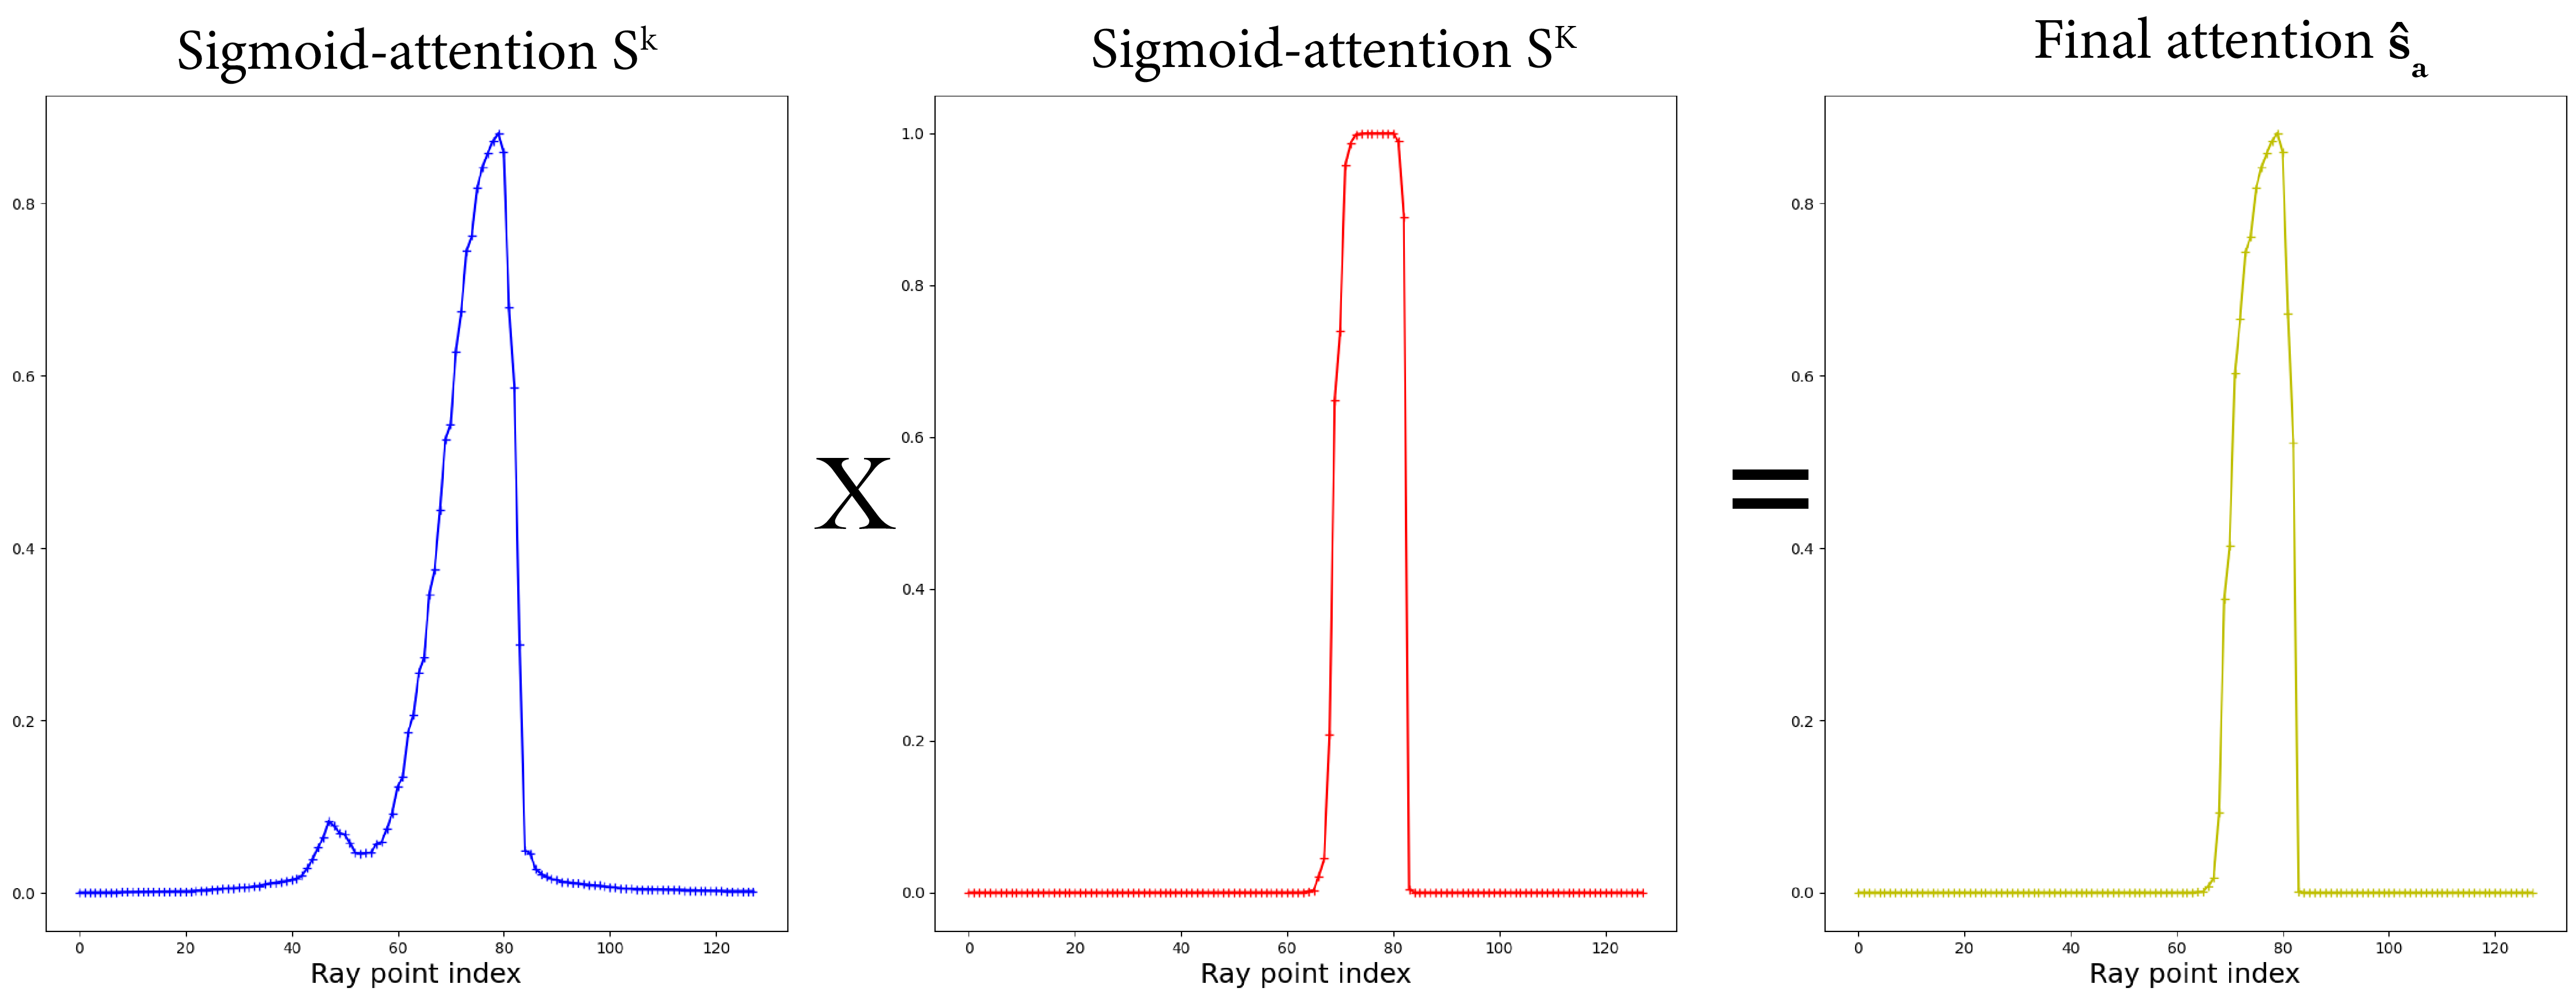
\includegraphics[width=\linewidth]{images/epinerf/SUPP_ATT_OVERLEAF.png}
  \caption{\textbf{Sigmoid shrinkage influence over} $\textbf{s}_{a}$. Intermediate attention distributions $S^{k}$ (\textit{left}) and $S^{K}$ (\textit{center}) allow to get $\hat{\mathbf{s}_{a}}$ (\textit{right}), the final attention distribution involved in the EpiNeRF architecture.}
  \label{fig:attention_sigmoid}
  \end{center}
\end{figure}

We finally illustrate on Figure \ref{fig:attention_construction} the $\alpha$-blending operation we performed in Chapter ~\ref{chapter:epinerf} through the Equation \ref{eq:alpha}. 

\begin{figure}[h!]
    \begin{center}
  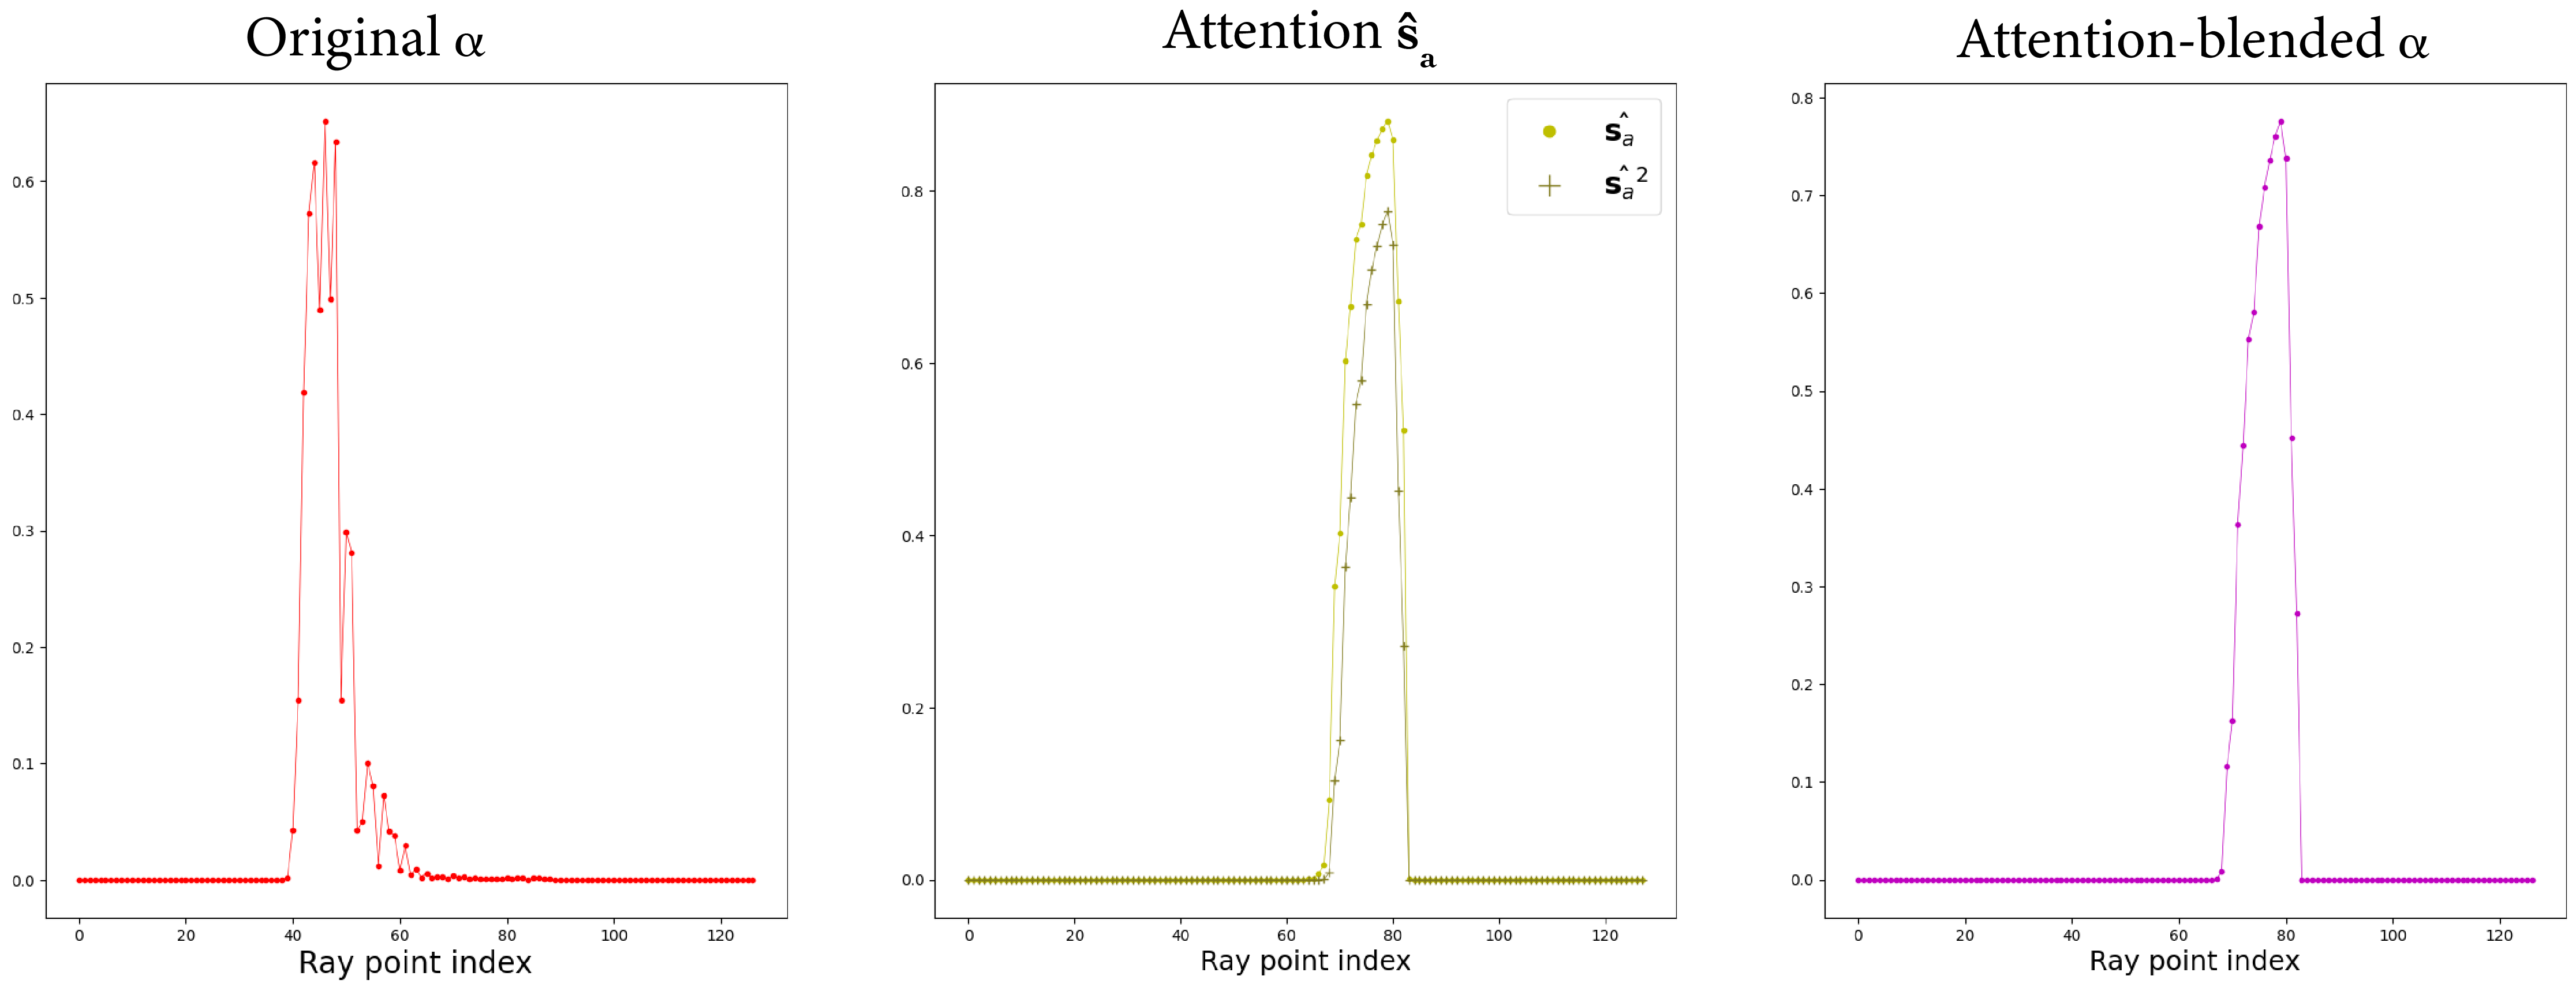
\includegraphics[width=\linewidth]{images/epinerf/SUPP_BLENDED_OVERLEAF.png}
  \caption{$\alpha$\textbf{-blending correction.} Original $\alpha$ distribution (\textit{left}) and its corrected attention-based counterpart (\textit{right}) show different activation regions along the ray. Cross-attention distributions $\hat{\textbf{s}}_{a}$ and $\hat{\textbf{s}}_{a}^{2}$ are plotted in the \textit{center} panel.}
  \label{fig:attention_construction}
  \end{center}
\end{figure}

The EpiNeRF epipolar cross-attention module aims to focus on regions where the attention $\hat{\textbf{s}}_{a}$ reaches its maximum values. As observed in Figure \ref{fig:attention_construction}, the blending operation shifts the $\alpha$ distribution slightly further away along the ray than it was originally. As expressed in Equation \ref{eq:weights} and illustrated in the devoted chapter with the Figure \ref{fig:overall_attention}, the transmittance $T$ is naturally affected by this shift correction. 

\subsection{Training details}
\label{appendix:epinerf-training}
Although our EpiNeRF architecture requires several intermediate training steps, we expand the training losses already expressed in Equations \ref{eq:nerfeature_loss} and \ref{eq:epinerf_loss}. Regarding NeRFeature, the L2-loss is given by: 

\begin{equation}
\begin{split}
 \mathcal{L}_{\Psi}&= \sum_{\mathbf{r}\in\mathcal{R}} || f_{t}(\mathbf{r}) - \underbrace{f_{t}^{(GT)}(\mathbf{r})}_{=\mathbf{F}_{t}(\pi(\mathbf{r}))} ||_{2}^{2} 
\end{split}
\end{equation}

with $\mathbf{F}_{t} = \chi(I_{t})$. The final target-aligned deep feature $f_{t}$ is expressed in Equation \ref{eq:ft_vr}. \newline

Concerning EpiNeRF final training, we get the loss function: 

\begin{equation}
\begin{split}
 \mathcal{L}_{\zeta}= \sum_{\mathbf{r}\in\mathcal{R}} || \hat{c}(\mathbf{r}) - \underbrace{c^{(GT)}(\mathbf{r})}_{= I_{t}(\pi(\mathbf{r}))} ||_{2}^{2}
\end{split}
\end{equation}
with $\zeta = \{\chi,\Phi,\Gamma\}$. Predicted colour $\hat{c}(\mathbf{r})$ can be decomposed through the volumetric rendering equation as: 

\begin{equation}
\hat{c}(\mathbf{r}) = \sum_{X^{(i)} \in \mathbf{r}}T^{(i)}\alpha^{(i)}c(\mathbf{X}^{(i)},\mathbf{d},\underbrace{f_{s}^{(i)},f_{s,symm}^{(i)}}_{= \mathbf{F}_{s}(\pi(X^{(i)})), \mathbf{F}_{s}(\pi(\mathbf{M}X^{(i)}))})
\end{equation}
with
\begin{equation}
\alpha^{(i)} = \hat{s}_{a}(1-\exp^{-\sigma(\mathbf{X}^{(i)})\delta_{i}}) + \hat{s}_{a}^{2}(\exp^{-\sigma(\mathbf{X}^{(i)})\delta_{i}}) \\
\end{equation}
the $\alpha$ blended distribution with our attention distribution $\hat{s}_{a}$, as expressed in Equation \ref{eq:alpha}. 

From a hyperparameter setting perspective, we follow the training strategy used in  SymmNeRF \citep{li2022symmnerf} and VisionNeRF \citep{lin2023vision} for $\chi$ and $\Phi$ and formed batches of 4 images during training. We averaged our loss function over 256 rays.

\section{Pseudo codes}

Pseudo codes related to the EpiNeRF training are provided below. 

Algorithm \ref{alg:one} outlines the training of the 2D \ac{CNN} encoder $\chi$ within a single-image \ac{NeRF}-based \ac{NVS} pipeline. This first pseudo-code thus includes both $\Phi$ and $\Gamma$ networks. Feature from the 2D \ac{CNN} encoder-decoder $\chi$ are then distilled into 3D feature radiance fields in Algorithm \ref{alg:two}. Finally, the EpiNeRF architecture is fine-tuned in Algorithm \ref{alg:fourth} thanks to our epipolar-based feature attention mechanism. Note that in this last pseudo-code, our epipolar feature-attention module is only activated in the coarse NeRF network. Once the coarse weights distribution is corrected by the epipolar feature-attention module, the fine-NeRF benefits from a more accurate distribution for sampling points. We have found that this implementation choice also helps make EpiNeRF training faster.

\begin{algorithm}[htbp]
    \caption{Joint pre-training of CNN $\chi$, NeRF $\Phi$, Hypernetwork $\Gamma$ }\label{alg:one}
    \SetKwInOut{Input}{input}
    \SetKwInOut{Parameter}{parameter}
    \SetKwInOut{Output}{output}
    \Input{Image pairs $\{I_{s},I_{t}\}$}
    \Parameter{\textbf{M} symmetry matrix on (YZ) plane}
    \Output{Trained $\zeta=\{\chi,\Phi,\Gamma\}$} 
    \medskip
    \KwResult{$\chi$ trained to produce view-aligned features}
    $N_{iter},\hspace{.1cm} N_{s},\hspace{.1cm} N_{rays},\hspace{.1cm}b_{s} \gets 500{,}000,\hspace{.1cm} 64,\hspace{.1cm} 256,\hspace{.1cm} 4$ \tcp*[l]{Training hyperparameters}
    $d_{\text{feat}} \gets 256$\;
    \While{$j \leq N_{iter}$}{
        \textcolor{red!50}{[FORWARD PASS]}\;
         $z_{s}\hspace{.05cm}, \textbf{F}_{s}  \gets \chi(I_{s})$ \hspace{3cm}\textcolor{gray!80}{\# 
       [bs,$d_{\text{feat}}$] , [bs,H,W,$d_{\text{feat}}$]}\;
        $\theta = \Gamma(z_{s})$ \tcp*{HyperNetwork $\Gamma$ forward pass}
        $\mathbf{r}(t) \gets \mathbf{o} + t\mathbf{d}$ \tcp*{Cast ray from target viewpoint}
            \For{$1 \leq i \leq N_{s}$}{
            $x^{(i)} \gets \mathbf{o} + t_{i}\mathbf{d}$\hspace{3cm}\textcolor{gray!80}{\# 
      [bs,$N_{rays}$,$N_{s}$]}\; 
            $x^{(i)}_{symm} \gets \mathbf{M}x^{(i)}$\tcp*{3D samples symmm. (YZ) plane}
            $f_{s}^{(i)} \gets \textbf{F}_{s}(\pi(x^{(i)}))$ \tcp*{Get source-aligned feature from $F_{s}$}
            $f_{s,symm}^{(i)} \gets \textbf{F}_{s}(\pi(x^{(i)}_{symm}))$ \tcp*{$f_{s}^{(i)}$ symmetrized counterpart}
            $f^{(i)} = [f_{s}^{(i)} \mid f_{s,symm}^{(i)}]$\tcp*{Concatenation}
        
            $\sigma^{(i)},\mathbf{c}^{(i)} \gets \Phi_{\theta}(x^{(i)},\mathbf{d},f_{s}^{(i)})$ \tcp*{NeRF $\Phi$ forward pass}
            }
            $c \gets \sum_{i=1}^{N_{s}} T_{\sigma}^{(i)}(1-\exp(-\delta_{i}\sigma^{(i)}))\textbf{c}^{(i)}$ \textcolor{gray!80}{\# 
      [bs,$N_{rays}$,3]} \tcp*{Vol. rendering}
      \;
      \textcolor{red!50}{[BACKWARD PASS]}\;
        $\zeta = \{\chi,\Phi,\Gamma\}$ \tcp*{Trainable architectures }
        $\mathcal{L}_{\zeta}= \sum_{\mathbf{r}\in\mathcal{R}} || c(\mathbf{r}) - c^{(GT)}(\mathbf{r}) ||_{2}^{2}$\tcp*{Training loss }
        $\Theta_{\zeta} \gets AdamW(\theta_{\zeta},\nabla_{\theta_{\zeta}} \mathcal{L}_{\zeta})$ \tcp*{Backpropagation - Weights update}
        }
    \end{algorithm}
 
\begin{algorithm}[htbp]
\caption{Training of NeRFeature $\Psi$ via $\chi$ feature distillation }\label{alg:two}
\SetKwInOut{Input}{input}
\SetKwInOut{Arch}{Freezed}
\SetKwInOut{Output}{output}
\SetKwInOut{Parameter}{parameter}
\Input{Image pairs $\{I_{s},I_{t}\}$}
\Parameter{Intrinsic camera parameters ($3\times3$ matrix) $K$}
\Arch{CNN encoder/decoder $\chi$ }
\Output{Trained NeRFeature $\Psi$ } 
\medskip
\KwResult{$\Psi$ trained to produce target-aligned features $f_{t} \in \mathbb{R}^{d_{\text{feat}}}$ from source-aligned ones.}
$N_{iter},\hspace{.1cm} N_{s},\hspace{.1cm} N_{rays},\hspace{.1cm}b_{s} \gets 300.000,\hspace{.1cm} 96,\hspace{.1cm} 256,\hspace{.1cm} 4$ \tcp*[l]{Training hyperparameters}
$d_{\text{feat}} \gets 256$\;
\While{j $\leq N_{iter}$}{
    \textcolor{red!50}{[FORWARD PASS]}\;
        \textunderscore \hspace{.05cm}, $\textbf{F}_{s}  \gets \chi(I_{s})$ \hspace{3cm}\textcolor{gray!80}{\# 
  [bs,H,W,$d_{\text{feat}}$]}\;
         \textunderscore \hspace{.05cm}, $\textbf{F}_{t}  \gets \chi(I_{t})$\;
         $\mathbf{r}(t) \gets \mathbf{o} + t\mathbf{d}$ \tcp*{Cast ray from target viewpoint}
        \For{$1 \leq i \leq N_{s}$}{
        $x^{(i)} \gets \mathbf{o} + t_{i}\mathbf{d}$\hspace{3cm}\textcolor{gray!80}{\# 
  [bs,$N_{rays}$,$N_{s}$]}\; 
        $f_{s}^{(i)} \gets \textbf{F}_{s}(\pi(x^{(i)}))$ \tcp*{Get source-aligned feature from $F_{s}$}
        $\rho^{(i)},\mathbf{v}^{(i)}_{t} \gets \Psi(x^{(i)},\mathbf{d},f_{s}^{(i)})$ \tcp*{NeRFeature $\Psi$ forward pass}
        }

        $f_{t} \gets \sum_{i=1}^{N_{s}} T_{\rho}^{(i)}(1-\exp(-\delta_{i}\rho^{(i)}))\textbf{v}^{(i)}_{t}$ \textcolor{gray!80}{\# 
  [bs,$N_{rays}$,$d_{\text{feat}}$]} \tcp*[l]{Vol. rendering}
  \;
  \textcolor{red!50}{[BACKWARD PASS]}\;
    $\mathcal{L}_{\Psi}= \sum_{\mathbf{r}\in\mathcal{R}} || f_{t}(\mathbf{r}) - f_{t}^{(GT)}(\mathbf{r}) ||_{2}^{2}$\tcp*{Loss - $f_{t}^{(GT)}(\mathbf{r}) =\mathbf{F}_{t}(K\mathbf{r})$}
    $\Theta_{\Psi} \gets AdamW(\theta_{\Psi},\nabla_{\theta_{\Psi}} \mathcal{L}_{\Psi})$ \tcp*{Backpropagation - Weights update}
    }
\end{algorithm}


\begin{algorithm}[htbp]
\caption{Fine-tunning of the complete EpiNeRF architecture including $\chi,\Gamma,\Phi$}\label{alg:fourth}
\SetKwInOut{Input}{input}
\SetKwInOut{Arch}{Freezed}
\SetKwInOut{PreTrained}{Pre-trained}
\SetKwInOut{Output}{output}
\SetKwInOut{Parameter}{parameter}
\Input{Image pairs $\{I_{s},I_{t}\}$}
\Parameter{\textbf{M} symmetry matrix on (YZ) plane}
\Arch{CNN encoder/decoder $\chi$, NeRFeature $\Psi$ }
\PreTrained{$\zeta = \{\chi,\Phi,\Gamma\}$ (Alg. 1) }
\Output{$\zeta = \{\chi,\Phi,\Gamma\}$ fine-tunned} 
\medskip
\KwResult{Final EpiNeRF model for single-image NVS}
$N_{iter},\hspace{.1cm} N_{s},\hspace{.1cm} N_{rays},\hspace{.1cm}b_{s} \gets 100.000,\hspace{.1cm} 64,\hspace{.1cm} 256,\hspace{.1cm} 4$ \tcp*[l]{Training hyperparameters}
$d_{\text{feat}} \gets 256$\;
\While{j $\leq N_{iter}$}{
    \textcolor{red!50}{[FORWARD PASS]}\;
        $z_{s}$ \hspace{.05cm}, $\textbf{F}_{s}  \gets \chi(I_{s})$ \hspace{3cm}\textcolor{gray!80}{\# 
  [bs,H,W,$d_{\text{feat}}$]} \tcp*[l]{(Alg. 1)}
         $\mathbf{r}(t) \gets \mathbf{o} + t\mathbf{d}$ \tcp*{Cast ray from target viewpoint}
         $\theta = \Gamma(z_{s})$ \tcp*{HyperNetwork $\Gamma$ forward pass}
        \textcolor{orange!50}{[Coarse NeRF $\Phi$]}\;
        \For{$1 \leq i \leq N_{s}$}{
        $x^{(i)} \gets \mathbf{o} + t_{i}\mathbf{d}$\hspace{3cm}\textcolor{gray!80}{\# 
  [bs,$N_{rays}$,$N_{s}$]}\tcp*{$t_{i}\sim$\textit{Uniform}}
        $x^{(i)}_{symm} \gets \mathbf{M}x^{(i)}$\tcp*{3D samples symmm. (YZ) plane}
        $f^{(i)} = [f_{s}^{(i)} || f_{s,symm}^{(i)}]$\tcp*{Source aligned features concatenation}
        
        $f_{t} \gets \Psi(x^{(i)},\mathbf{d},f_{s}^{(i)})$ \tcp*{NeRFeature $\Psi$ forward pass. (Alg. 2)}
        $s_{a}^{(i)} = \frac{f_{t}^{T}\times f_{s}^{(i)}}{\sqrt{d_{\text{feat}}}}$\textcolor{gray!80}{ $\in$[0,1]} \tcp*{Cross-attention score}
        $\sigma^{(i)},\mathbf{c}^{(i)} = \Phi_{\theta}(x^{(i)},\mathbf{d},f^{(i)})$ \tcp*{Coarse NeRF $\Phi$ forward pass}
        $\alpha^{(i)} \gets  \alpha^{(i)}s_{a}^{(i)} + (1-\alpha^{(i)})s_{a}^{(i)^{2}}$ \tcp*{Attention blending}
        
        $\omega^{(i)} = T_{\sigma}^{(i)}\alpha^{(i)}$  \tcp*{Attention-corrected weights distribution}
        }
        \;
        $c_{coarse} = \sum_{i=1}^{N_{s}}\omega^{(i)}\textbf{c}^{(i)}$ \tcp*{Coarse volume rendering}
        $t_{i}\sim F^{-1}(u)$ \tcp*{Impor. samp.
 of CDF $F(j)=\sum_{i=1}^{j}\omega_{i}$, $u\sim$\textit{Uniform}}
        \;
        \textcolor{orange!50}{[Fine NeRF $\Phi$]}\;
        \For{$1 \leq i \leq N_{s}$}{
        $x^{(i)} \gets \mathbf{o} + t_{i}\mathbf{d}$ 
        $x^{(i)}_{symm} \gets \mathbf{M}x^{(i)}$\tcp*{3D samples symmm. (YZ) plane}
        
        $f^{(i)} = [f_{s}^{(i)} | f_{s,symm}^{(i)}]$\tcp*{Source aligned features concatenation}
        $\sigma^{(i)},\mathbf{c}^{(i)} = \Phi_{\theta}(x^{(i)},\mathbf{d},f^{(i)})$ \tcp*{Fine NeRF $\Phi$ forward pass}
        $\omega^{(i)} = T_{\sigma}^{(i)}\alpha^{(i)}$ 
        }
        $c_{fine} = \sum_{i=1}^{N_{s}}\omega^{(i)}\textbf{c}^{(i)}$ \tcp*{Fine volume rendering}
  \;
  \textcolor{red!50}{[BACKWARD PASS]}\;
    $\mathcal{L}_{\zeta}= \sum_{\mathbf{r}\in\mathcal{R}} || c_{coarse}(\mathbf{r}) - c^{(GT)}(\mathbf{r}) ||_{2}^{2} +|| c_{fine}(\mathbf{r}) - c^{(GT)}(\mathbf{r}) ||_{2}^{2}$\tcp*{Loss}
    $\Theta_{\zeta} \gets AdamW(\theta_{\zeta},\nabla_{\theta_{\zeta}} \mathcal{L}_{\Psi})$ \tcp*{Backpropagation - Weights update}
    }
\end{algorithm}


\section{Additional results - SRN dataset }
\label{appendix:moreres-epinerf}

The results shown on Figures \ref{fig:supp_NVScars} and \ref{fig:supp_NVSchairs} depict  sharp novel views synthesis, even from viewpoints far away from the source. 

\begin{figure}[htp!]
   \begin{center}
  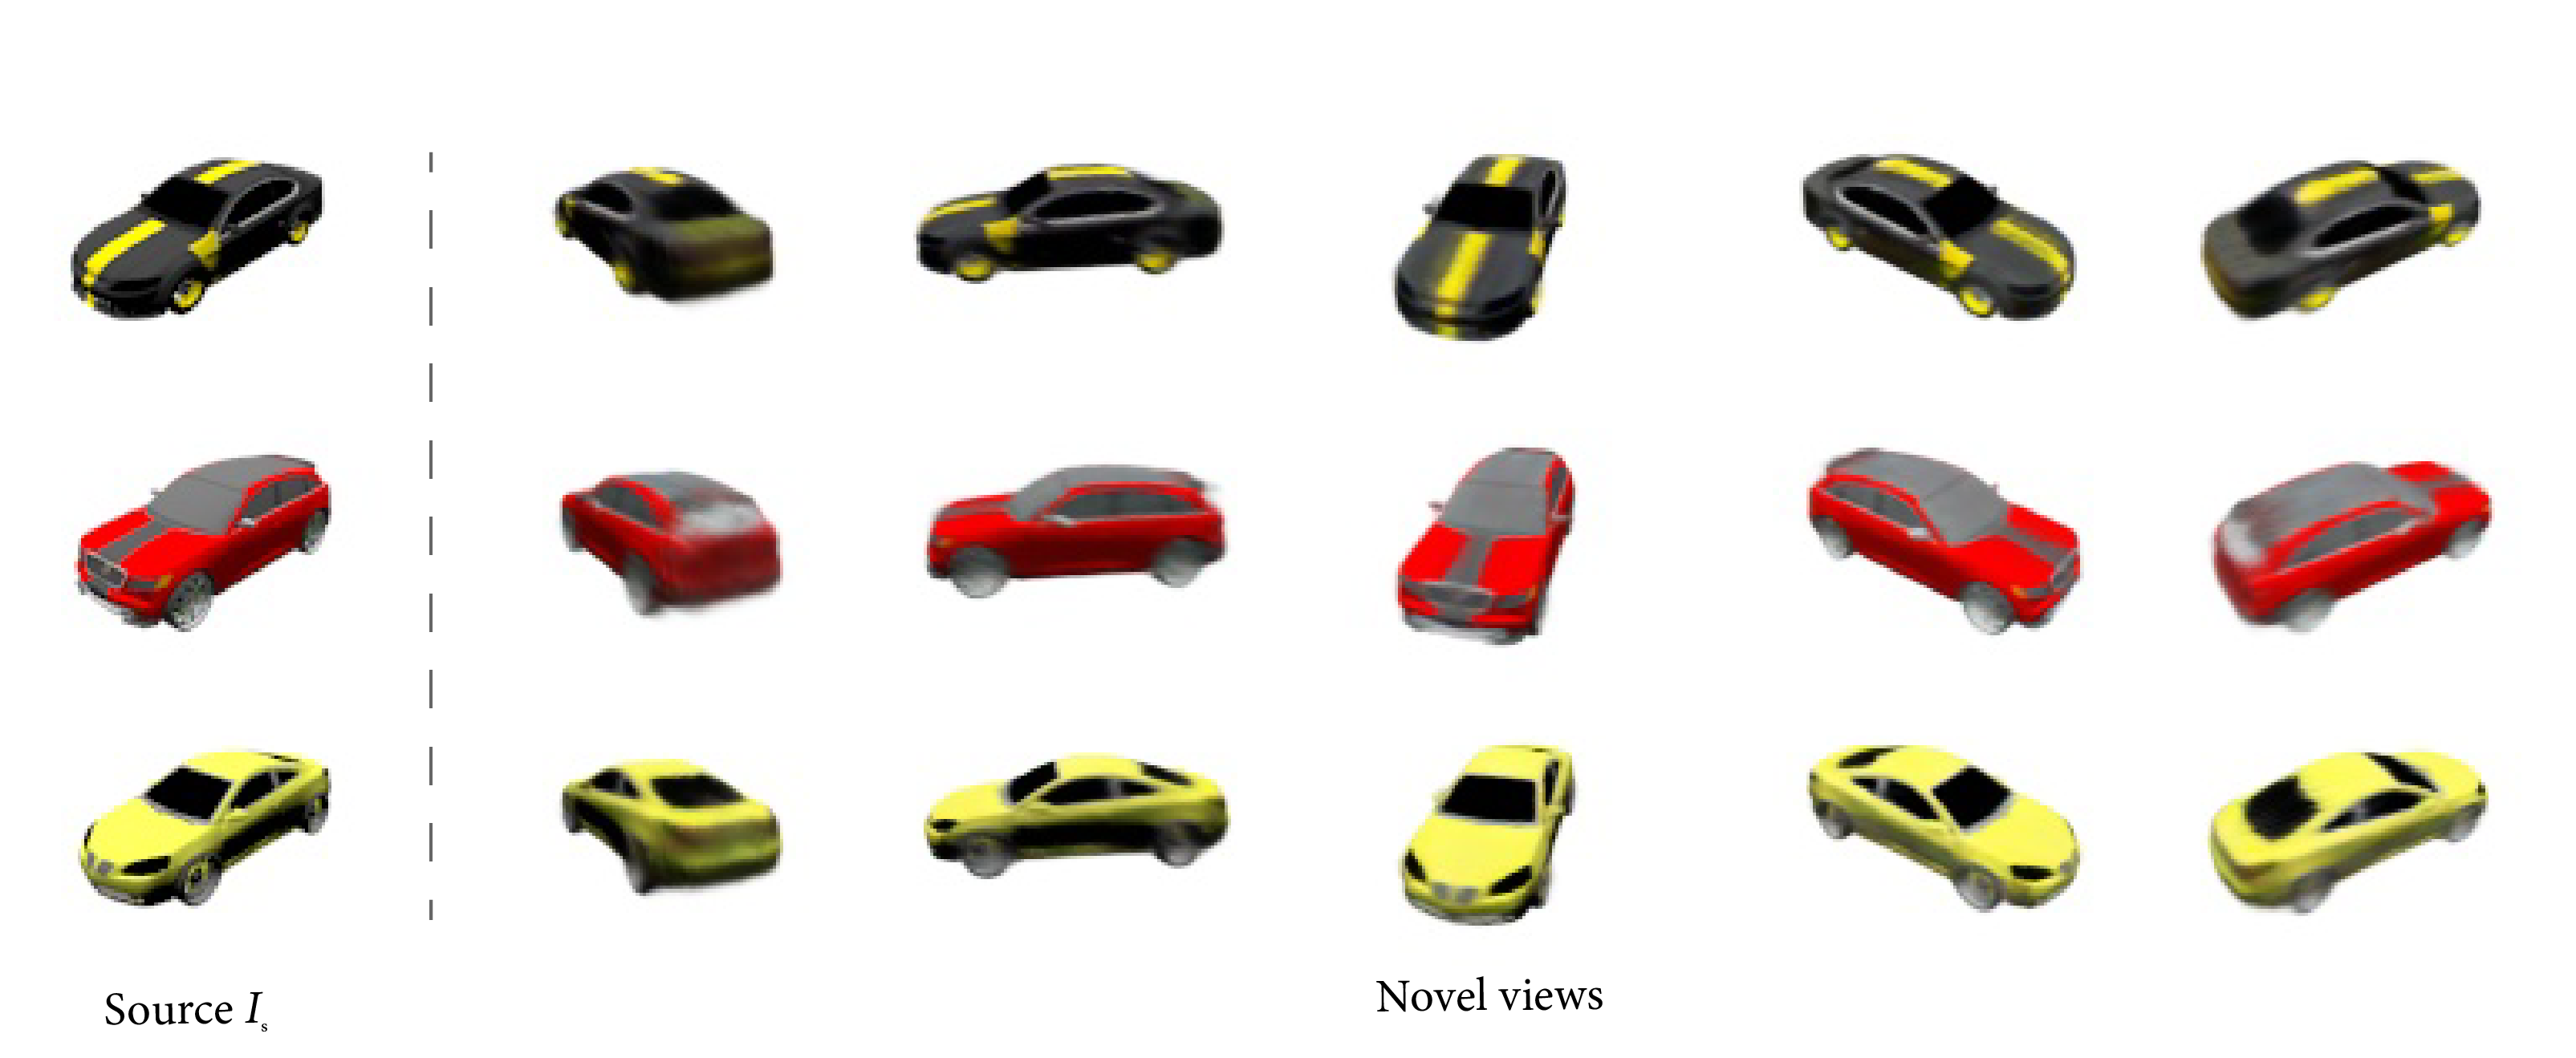
\includegraphics[width=\linewidth]{images/epinerf/supp_NVS_Cars.png}
  \caption{\textbf{Novel view synthesis.} Additional views on ShapeNet-SRN \textit{Cars} class are rendered from a broad range of viewpoints given a single source image. }
  \label{fig:supp_NVScars}
  \end{center}
\end{figure}


\begin{figure}[htp!]
    \begin{center}
  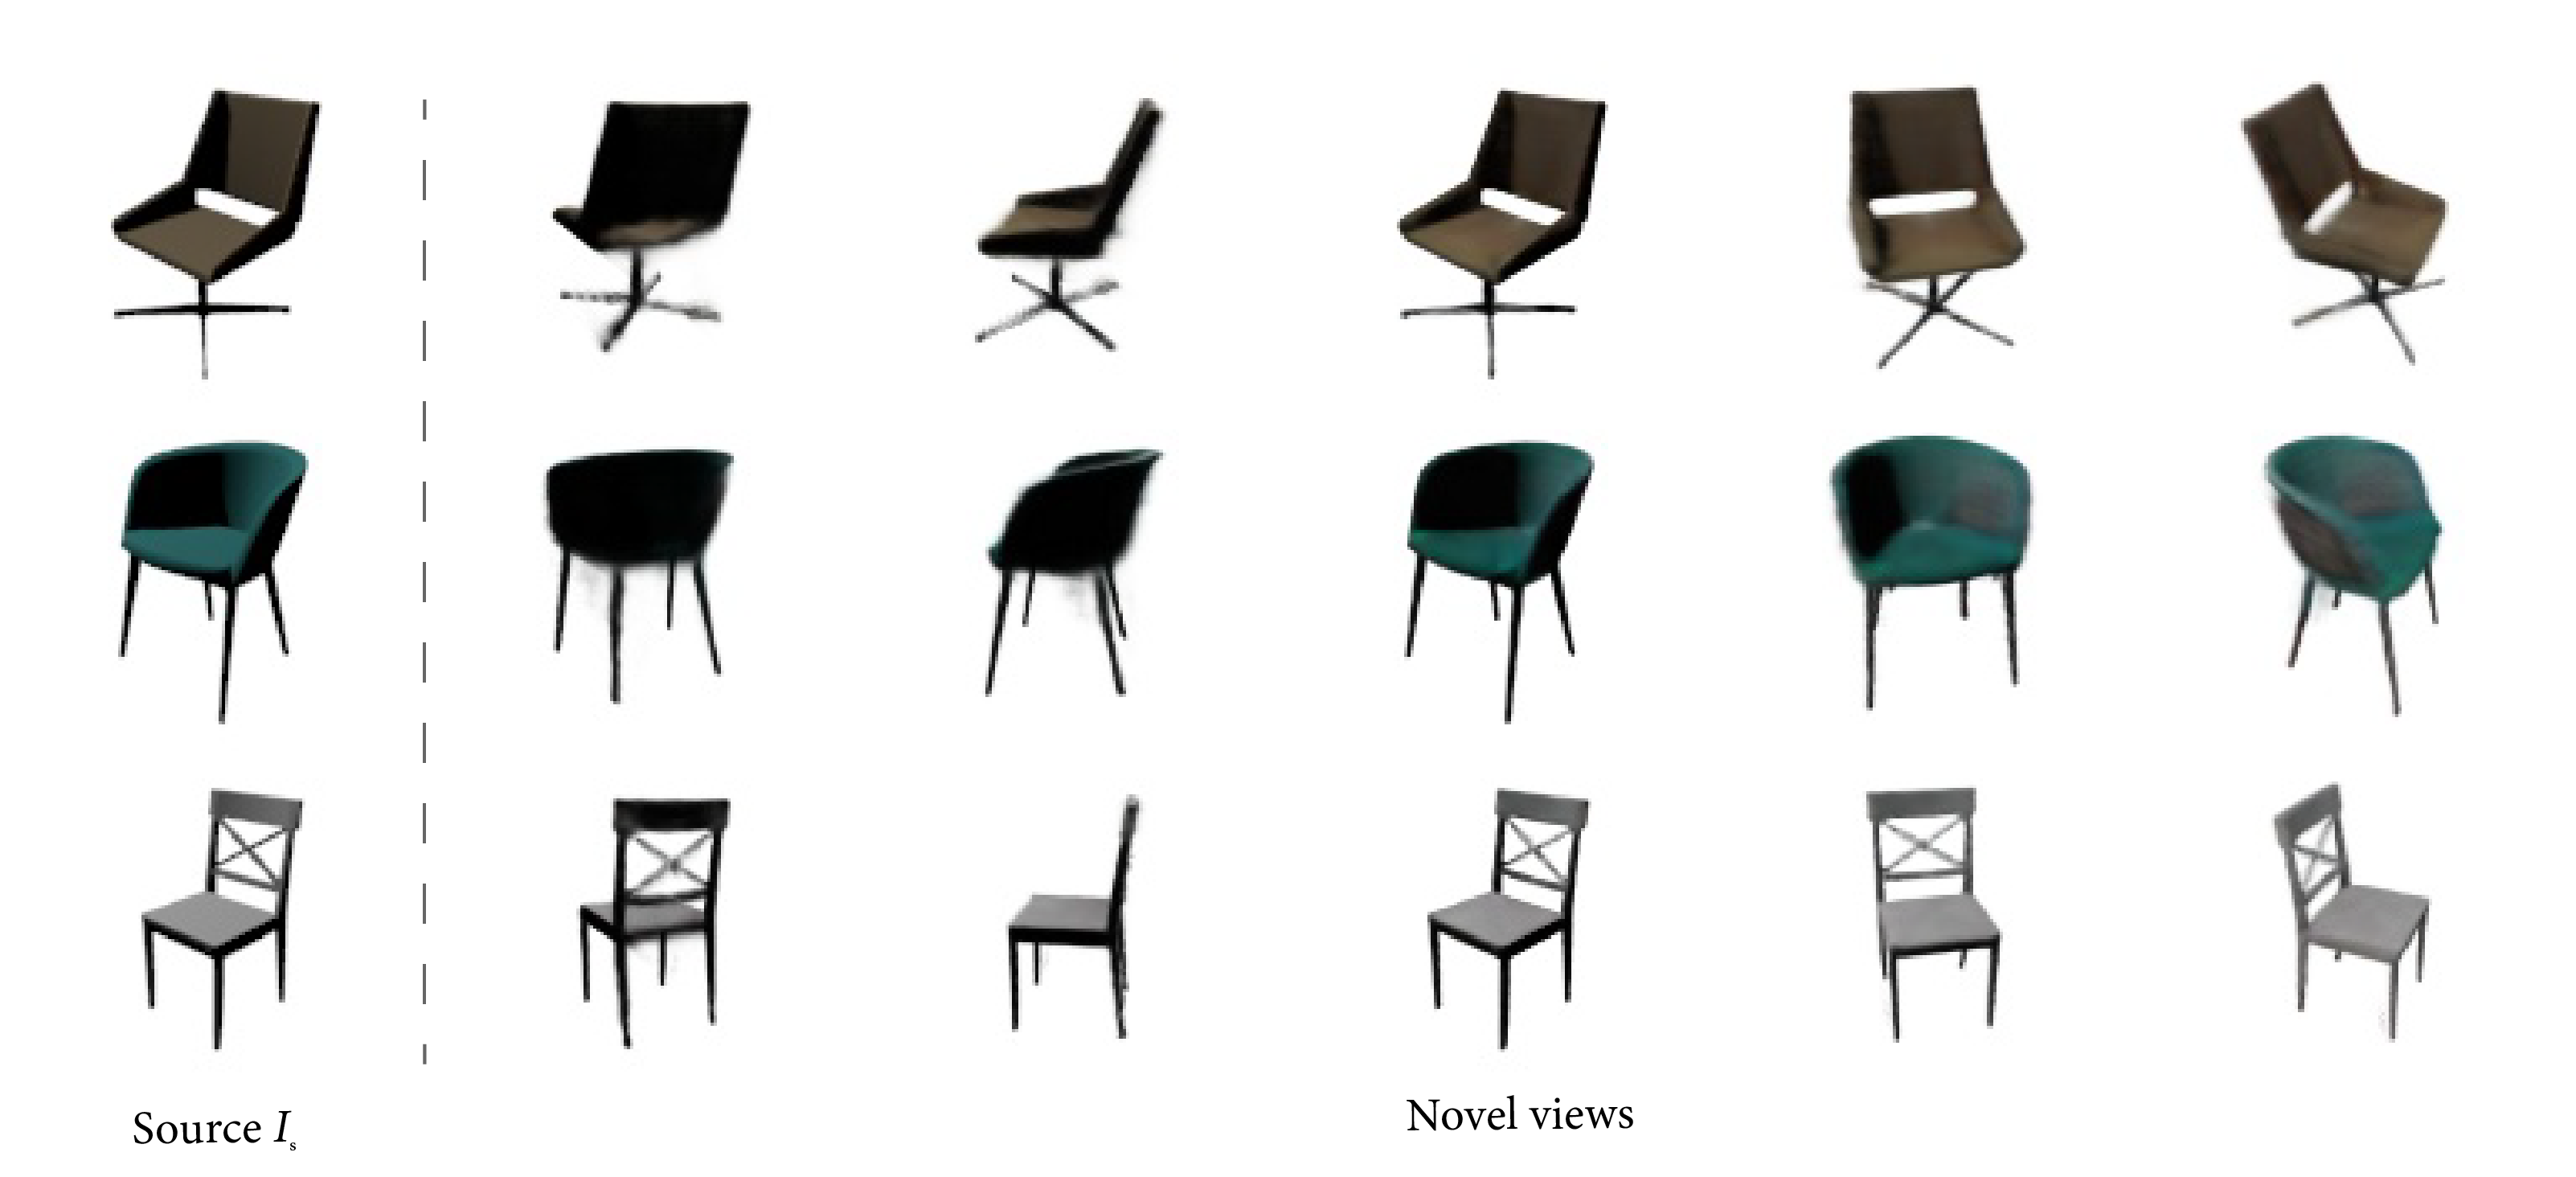
\includegraphics[width=\linewidth]{images/epinerf/supp_NVS_Chairs.png}
  \caption{\textbf{Novel view synthesis.} Additional views on ShapeNet-SRN \textit{Chairs} class are rendered from a broad range of viewpoints given a single source image. }
  \label{fig:supp_NVSchairs}
  \end{center}
\end{figure}

Figures \ref{fig:supp_cars} and \ref{fig:supp_chairs} show additional side-by-side renderings against state-of-the-art methods. As mentioned in Chapter \ref{chapter:epinerf}, EpiNeRF managed to better handle occlusions or unseen parts in view generation compared to current state-of-the-art methods thanks to its consideration for target-aligned features. Armrests and door paintings are rendered with sharper details. EpiNeRF achieves these \ac{NVS} performances without requiring a large \ac{GPU} cluster for training, unlike VisionNeRF \cite{lin2023vision}.

\begin{figure*}[htp!]
    \begin{center}
  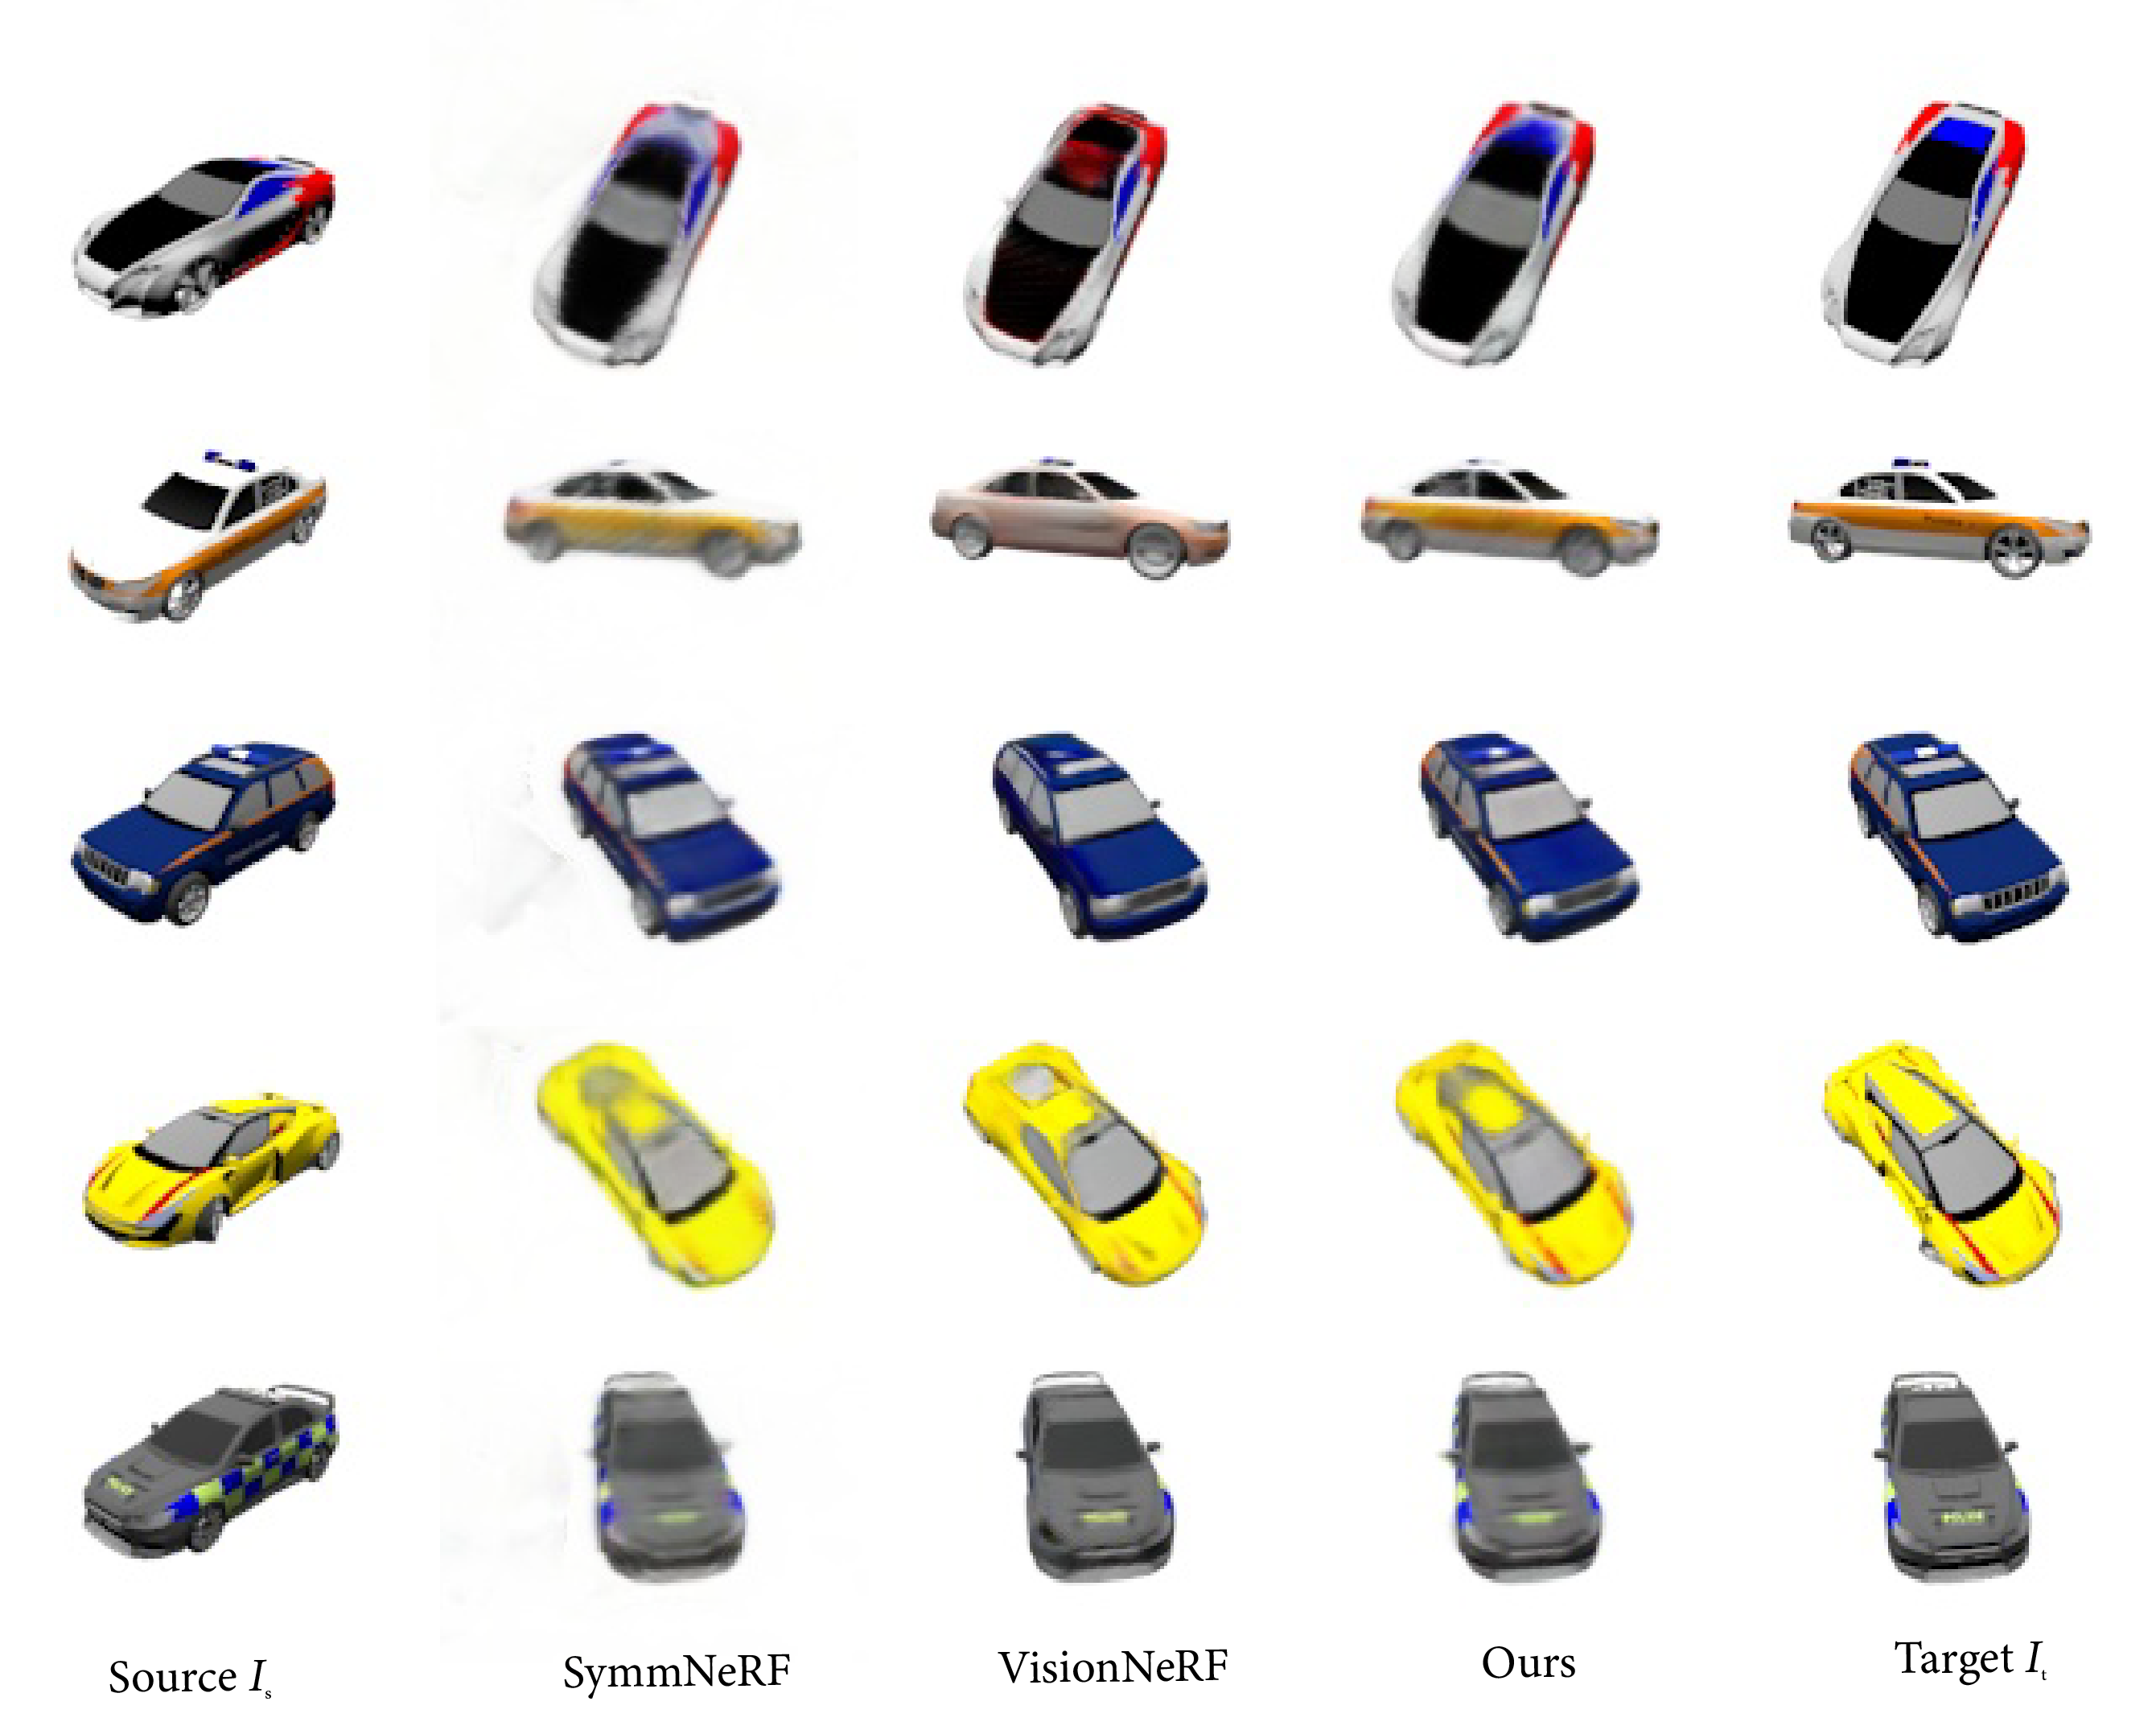
\includegraphics[width=\linewidth]{images/epinerf/supp_Cars_additional_inference.png}
  \caption{\textbf{Novel view synthesis on the ShapeNet category-specific} \textit{Cars. }EpiNeRF generates sharper views than SymmNeRF while preserving the symmetry aspects that VisionNeRF failed to maintain.}
  \label{fig:supp_cars}
  \end{center}
\end{figure*}


\begin{figure*}[htp!]
    \begin{center}
  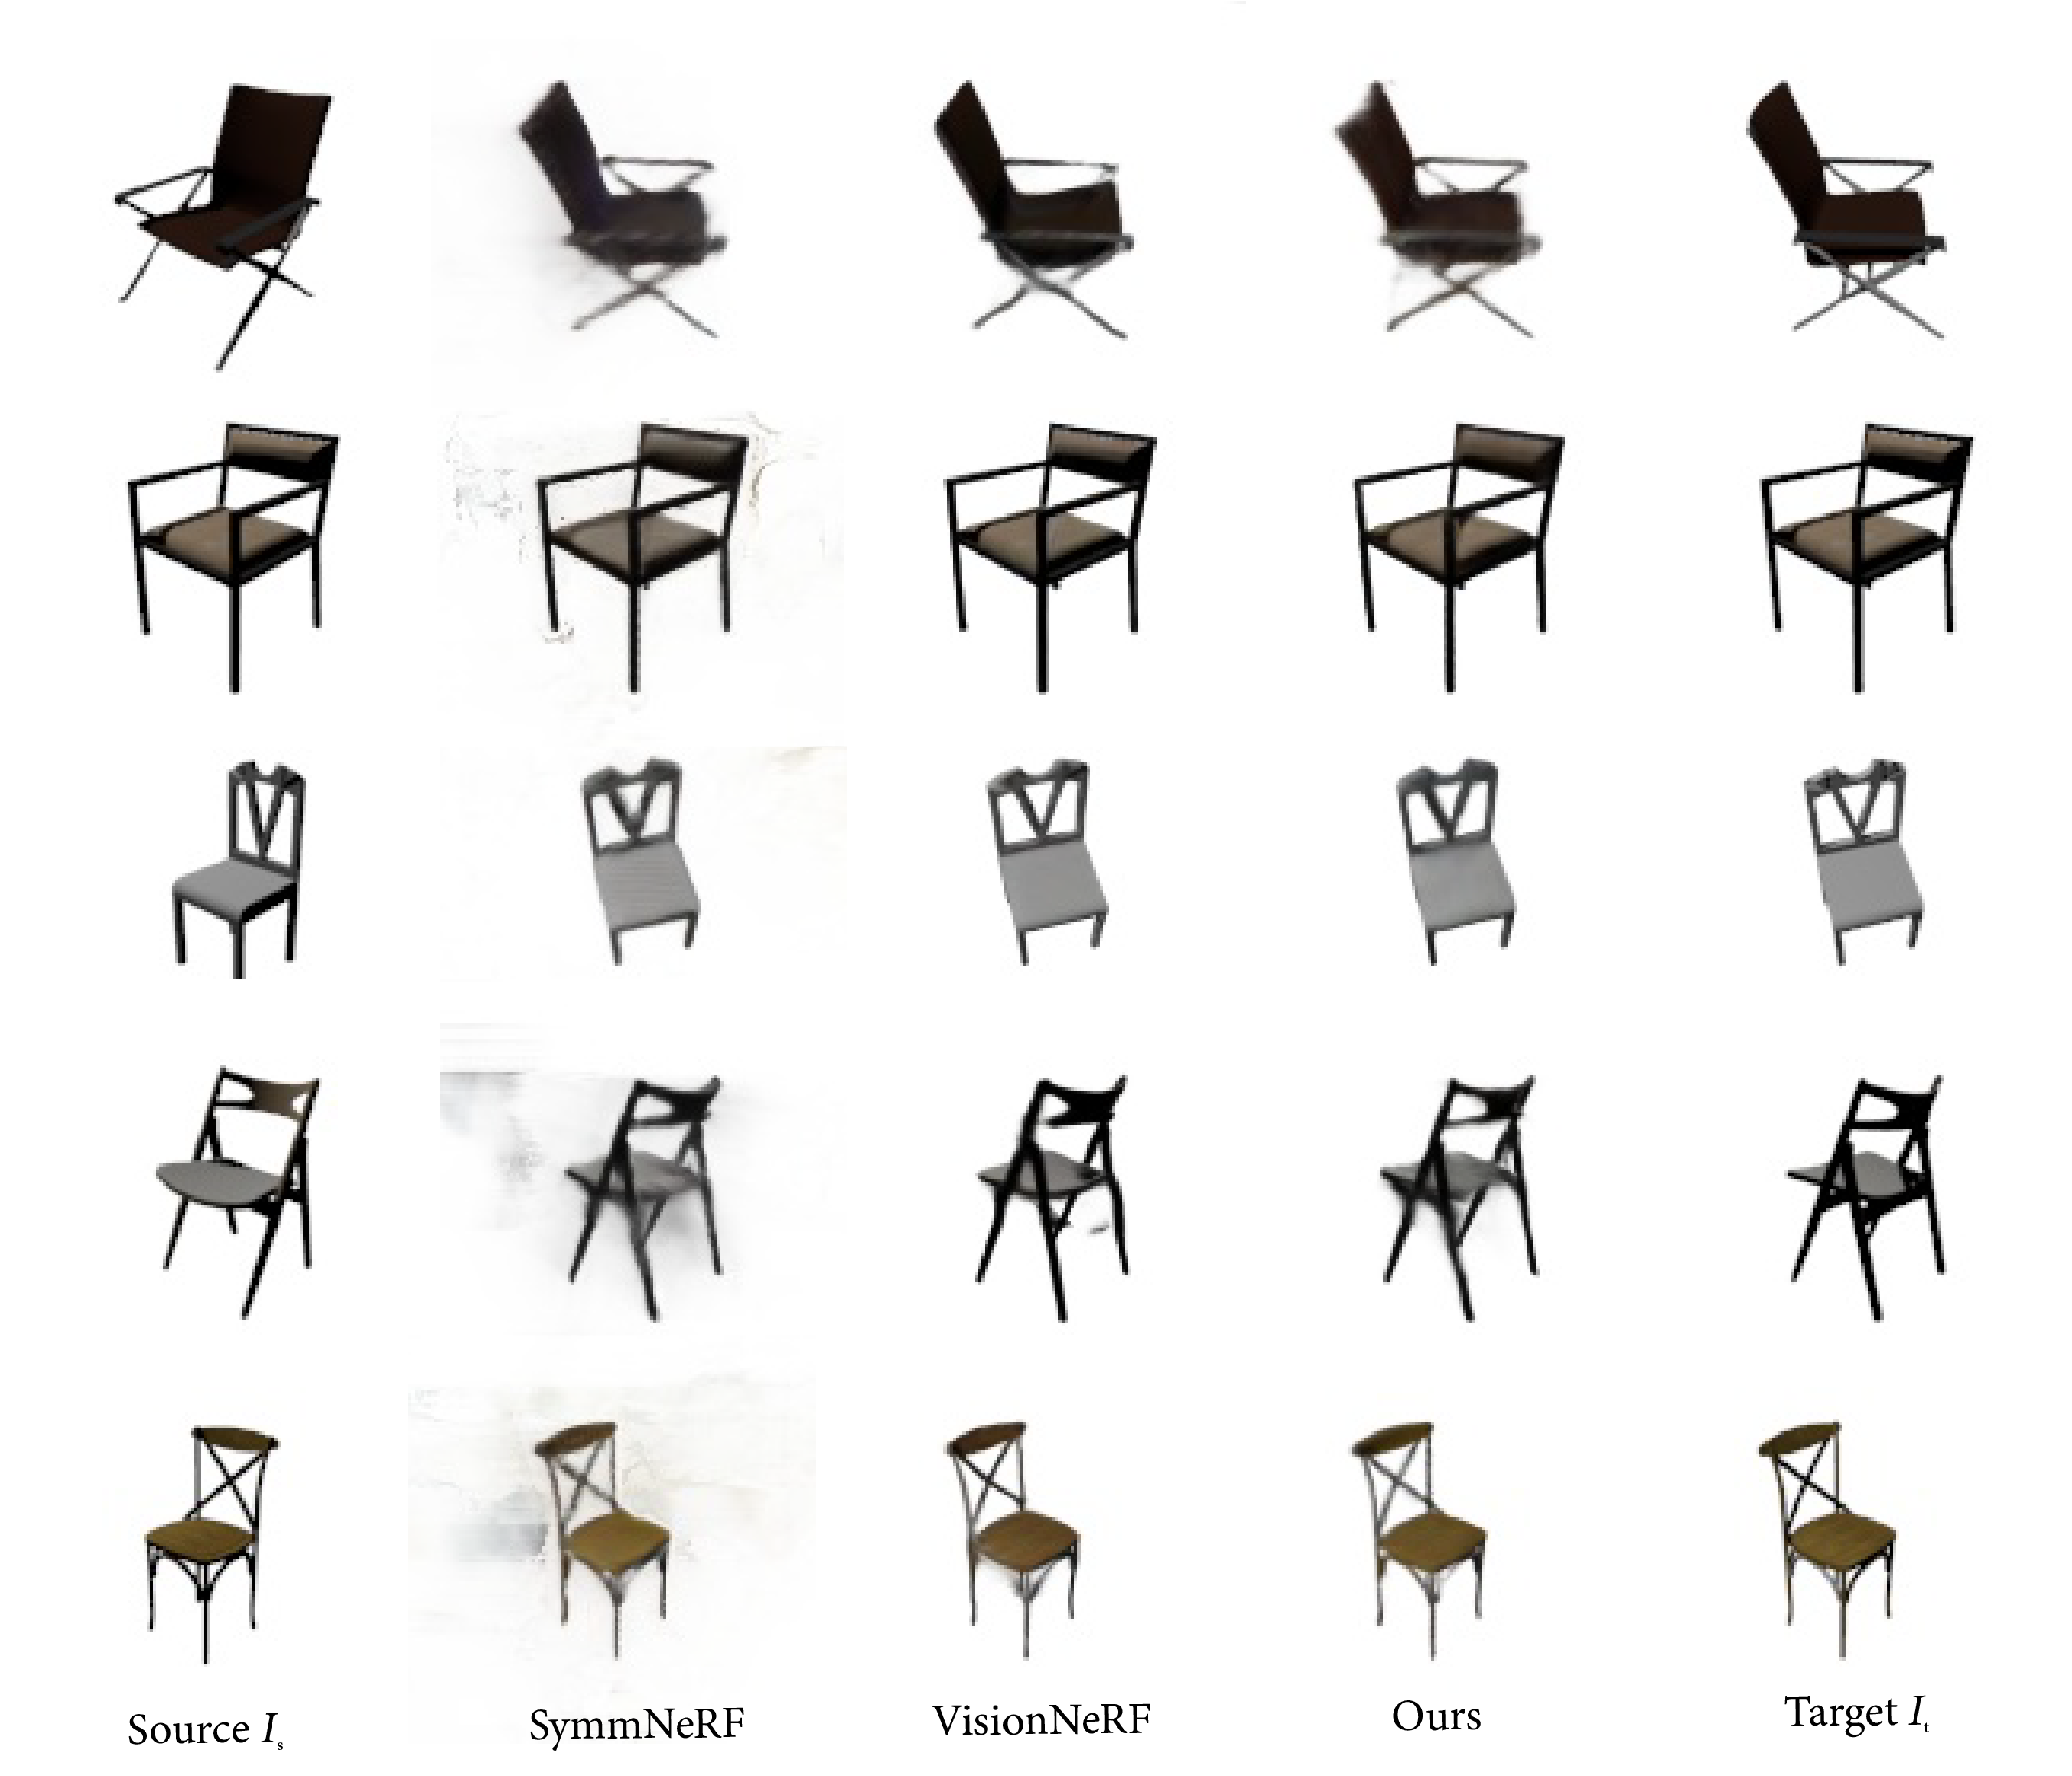
\includegraphics[width=\linewidth]{images/epinerf/supp_Chairs_additional_inference.png}
  \caption{\textbf{Novel view synthesis on the ShapeNet category-specific} \textit{Chairs. }EpiNeRF generates sharper views than SymmNeRF while preserving the symmetry aspects that VisionNeRF failed to maintain.}
  \label{fig:supp_chairs}
  \end{center}
\end{figure*}

\chapter{3DGS :Additional ressources}

We mostly present in this last section a few mathematical proofs concerning properties that were assumed in Chapter ~\ref{chapter:gausssplat}. 

\section{Gaussian primitives transformation}
\label{appendix:cov}
Let's first get into the Equation \ref{eq:gs-3dcov-transfrom} that transforms the 3D covariance $\Sigma^{(k)}_{3D}$ from world to camera coordinate system.

Given the linear transformation $R$ and the translation $t$, one can thus express any point $p$ in the world coordinate into its camera coordinate counter part through $p' = R\times p + t$. We thus also have the revert operation with: $p = R^{-1}\times (p' - t)$. 

The 3D gaussian primitive $\mathcal{G}_{k}$: 

\begin{equation}
    \mathcal{G}_{k}(p) = \exp \left(-\frac{1}{2}(p-\mu^{(k)}_{3D})^{T}(\Sigma^{(k)}_{3D})^{-1}(p-\mu^{(k)}_{3D})\right)
  \end{equation}
  
is thus transformed through: 
\begin{equation}
    \begin{aligned}
    \mathcal{G}_{k}(p) &= \exp \left( -\frac{1}{2} \{R^{-1}(p'-t) - R^{-1}(\mu^{(k)}_{cc} -t)\}^{T} (\Sigma^{(k)}_{3D})^{-1}\{R^{-1}(p'-t) - R^{-1}(\mu^{(k)}_{cc} -t)\}  \right) \\
    &= \exp \left( -\frac{1}{2}\{ R^{-1}(p'-\mu^{(k)}_{cc})\}^{T}(\Sigma^{(k)}_{3D})^{-1})\{ R^{-1}(p'-\mu^{(k)}_{cc})\} \right) \\
    &= \exp \left( -\frac{1}{2}(p'-\mu^{(k)}_{cc})^{T}R\times(\Sigma^{(k)}_{3D})^{-1}\times R^{-1}(p'-\mu^{(k)}_{cc})\right) \\
    &= \exp \left( -\frac{1}{2}(p'-\mu^{(k)}_{cc})^{T}(\Sigma^{(k)}_{3D})^{-1}(p'-\mu^{(k)}_{cc})\right) \\
    \end{aligned}
\end{equation}

with thus $\Sigma^{(k)}_{cc} = R\times \Sigma^{(k)}_{3D}\times R^{-1}$. \newline


Considering the affine approximation of $\phi$, we have from Equation \eqref{eq:affine_transform}: 

\begin{equation}
  \phi(p') - \phi(\mu_{cc}) \approx J(p' - \mu_{cc})
\end{equation}

and the primitive $\mathcal{G}_{k}$ is expressed in the ray space as: 

\begin{equation}
  \begin{aligned}
\mathcal{G}_{k}(\phi(p')) &= \exp \left( -\frac{1}{2}(\phi(p')-\phi(\mu^{(k)}_{cc}))^{T}(\Sigma^{(k)}_{3D})^{-1}(\phi(p')-\phi(\mu^{(k)}_{cc}))\right)\\
                        &= \exp \left( -\frac{1}{2}(J_{k}(p'-\mu^{(k)}_{cc}))^{T}(\Sigma^{(k)}_{3D})^{-1}(J_{k}(p'-\mu^{(k)}_{cc}))\right) \\
                        &= \exp \left( -\frac{1}{2}(p'-\mu^{(k)}_{cc})^{T}J_{k}^{T}(\Sigma^{(k)}_{3D})^{-1}J_{k}(p'-\mu^{(k)}_{cc})\right)\\
                        &= \exp \left( -\frac{1}{2}(p'-\mu^{(k)}_{cc})^{T}(J_{k}\Sigma^{(k)}_{3D}J_{k}^{T})^{-1}(p'-\mu^{(k)}_{cc})\right)
  \end{aligned}
\end{equation}

As explained in \citep{zwicker2001ewa}, one can drop the thrid row and column of  $\Sigma^{(k)}_{ic}$ to get a 2D covariance matrix, named $\Sigma^{(k)}_{2D}$. Applying a projective transformation to any 3D gaussian primitive $\mathcal{G}_{k}$ lead to the scaled 2D gaussian primitive, termed $g_{k}$: 

\begin{equation}
    g_{k}(x) = \exp(-\frac{1}{2}(x-\mu^{(k)}_{2D})^{T}(\Sigma^{(k)}_{2D})^{-1}(p-\mu^{(k)}_{2D}))
\end{equation}

with $\mu^{(k)}_{2D}= \phi(\mu_{cc}^{k})$ and $\Sigma^{(k)}_{2D}= J\Sigma^{(k)}_{cc}J^{T}$ the 2D mean and $2\times2$ covariance matric of $ g_{k}$. 


\section{Spherical Harmonics: How color is made view-dependent ?}
\label{appendix:gs-sh}

A gaussian primitive $\mathcal{G}_{k}$ do not store the color information through an RGB value. Authors from 3D\ac{GS} rather made color view-dependent by relying on \ac{SH} functions. 

The normalized viewing direction $\mathbf{d}$ we looking at can thus be expressed in spherical coordinates through the pair of angles $(\theta,\phi)$. From there, \ac{SH} functions are defined on sphere surface with \textit{l} bands and $-l \leq  m \leq l$ elementary functions $Y_{l}^{m}$ within each band.

\begin{equation}
    Y_{l}^{m}(\theta,\phi) = \frac{(-1)^{l}}{2^{l}l!} \times \sqrt{\frac{(2l+1)(l+m)!}{4\pi(l-m)!}}e^{im\phi}(sin(\theta))^{-m}\frac{d^{l-m}sin(\theta)^{2l}}{d(cos(\theta)^{l-m})}
\end{equation}

3D\ac{GS} usually considers 4 bands of \ac{SH}, and consider the view-dependent color $c$: 

\begin{equation}
    c(\mathbf{d}) = \sum_{l=0}^{3}\sum_{m=-l}^{m=l}k_{l}^{m}Y_{l}^{m}(\mathbf{d})
\end{equation}

while the $k_{l}^{m}$ are the \ac{SH}-coefficient that needs to be learned during training per gaussian primitives. 

\section{Undetermined positional gradient signs in the ADC}
\label{appendix:sign-gradient}

As mentioned in Section ~\ref{gs:pixgs-adc}, the per-pixel gradient $\frac{\partial L_{j}}{\partial \mu^{k}_{ndc,x}}$ is expressed as a sum of product terms that might have different signs. 

We thus already expressed such a per-pixel gradient for the x-axis as: 

\begin{equation}
    \label{eq:perpix-grad-appendix}
    \frac{\partial L_{j}}{\partial \mu^{k}_{ndc,x}} = \sum \limits_{l=1}^{3} \frac{\partial L_{j}}{\partial c_{l}^{j}}\times \frac{\partial c_{l}^{j}}{\partial \alpha_{k}^{j}} \times \frac{\alpha_{k}^{j}}{\partial \mu^{k}_{ndc,x} }
    \end{equation}

\begin{itemize}
    
    \item \textbf{First term} $\frac{\partial L_{j}}{\partial c_{l}^{j}}$ 
This partial derivative is rather straightforward as $\partial L_{j}$ define the $L_{1}$ loss function between the rendered pixel color and the ground truth one. This first term is thus either set to $+1$ or $-1$ and its sign is undertermined as soon as the difference between predicted and ground truth color can either be positive or negative. 

    \item \textbf{Second term} $\frac{\partial c_{l}^{j}}{\partial \alpha_{k}^{j}}$ 
The second term has to be developed to fully grasp why it also exists a sign ambiguity in its expression. Accounting on the expression of the rendered color in Equation \eqref{eq:gs-alpha-blending}, such partial derivative can thus be derived as follow. We drop here both the channel  \textit{l} as well as the pixel \textit{j} indexing for sake of clarity.  

\begin{equation}
    \frac{\partial c_{l}^{j}}{\partial \alpha_{k}} = c_{k} \times \prod \limits_{p=1}^{k-1}(1 - \alpha_{p}) - \sum \limits_{q=k+1}^{K} c_{q}\alpha_{q}\prod \limits_{p=1,p\neq q}^{q-1}(1 - \alpha_{p})
\end{equation}
Whearas both term are positives, their difference made such a term undetermined regarding its sign. 

    \item \textbf{Third term} $\frac{\partial \alpha_{k}^{j}}{\partial \mu^{k}_{ndc,x}}$ 
This last term can directly be derived from Equation \eqref{eq:gs-alpha-def}. We still drop the indexing $j$ for clarity and the aformentioned equation can be fully developped through: 
\begin{equation}
    \alpha_{k}(pix) =o_{k} \times g_{k}(pix) =  o_{k} \times \exp \left( -\frac{1}{2} \mathbf{d}^T \left( \Sigma_{2D}^{(k)} \right)^{-1} \mathbf{d} \right),  
\end{equation}
where $\mathbf{d} = \begin{pmatrix}
    p_x - \mu_{2D,x}^{(k)} \\
    p_y - \mu_{2D,y}^{(k)}
\end{pmatrix}$ and $pix=\left( p_{x},p_{y}\right)^{T}$ 

We thus get for the last partial derivative: 
\begin{equation}
    \frac{\partial \alpha_{k}}{\partial \mu^{(k)}_{ndc,x}} =  o_{k} \times \frac{\partial g_{k}}{\partial \mu^{k}_{ndc,x}} = o_{k} \times g_{k} \times ((\Sigma_{2D}^{(k)})^{-1}\mathbf{d})_{x}
\end{equation}
The sign of this third and last term thus directly depends on the sign of $\mathbf{d}_{x} = p_x - \mu_{2D,x}^{(k)}$, which is undetermined. 

\end{itemize}






